% \iffalse meta-comment
%
% File: hduthesis.dtx
% -----------------------------------------------------------------------
%   Copyright (C) 2023-2025 by Mingyu Xia <myhsia@outlook.com>          *
%                                                                       *
%   It may be distributed and/or modified under the conditions of the   *
%   LaTeX Project Public License (LPPL), either version 1.3c of this    *
%   license or (at your option) any later version. The latest version   *
%   of this license is in the file                                      *
%                                                                       *
%       http://www.latex-project.org/lppl.txt                           *
%                                                                       *
%   This work has the LPPL maintenance status `maintained'.             *
%                                                                       *
%   The Current Maintainer of this work is Mingyu Xia.                  *
%                                                                       *
%   This work consists of the files hduthesis.dtx,                      *
%                                   hdu-graphics.dtx,                   *
%                               and hduthesis.ins,                      *
%             and the derived files hduthesis.cls,                      *
%                                   hdu-<module>.code.tex,              *
%                                   beamerthemehdu.sty,                 *
%                                   hdulogo.pdf,                        *
%                                   hdutitle.pdf,                       *
%                                   hdubadge.pdf,                       *
%                                   hdumotto.pdf,                       *
%                                   hduthesis.pdf,                      *
%                               and README.md.                          *
% -----------------------------------------------------------------------
%
%   Any modification of this file should ensure that the copyright and
%   license information is placed in the derived files.
%
% -----------------------------------------------------------------------
%
%<*internal>
\iffalse
%</internal>
%
%<*readme>
The `hduthesis` Class: LaTeX class for Hangzhou Dianzi University
=================================================================

LaTeX class for bachelor and mphil theses in Hangzhou Dianzi
University is constructed by `LaTeX-expl3`. This class provides typesets
for bachelors' and mphils' thesis in Hangzhou Dianzi University.

Modules of `hduThesiS` provide the following supports:

- `typeset`: Math and text Typeset

- `layout`: Some central layout typeset interfaces

- `bc.config`: Configuration for bachelor thesis' style

- `pg.config`: Configuration for mphil thesis' style

- `beamer`: HDU Beamer theme

- `stationery`: Creation of HDU's stationery

- `exam`: Typeset for HDU examinations' solution

- `l3doc`: Configuration for class's `l3doc` manual

Issues
------

The issue tracker for `hduthesis` is currently located
[on GitHub](https://github.com/myhsia/hduthesis/issues).

---

杭州电子科技大学学位论文 LaTeX 模板
==============================

杭州电子科技大学学位论文 LaTeX 模板以 `LaTeX-expl3` 构建,提供杭州电子科技大学学士和硕士学位论文格式.

`hduThesiS` 的模块提供以下支持:

- `typeset`: 数学和文本排版

- `layout`: 封面和浮动题布局

- `bc.config`: 学士论文格式配置

- `pg.config`: 硕士论文格式配置

- `beamer`: HDU Beamer 主题

- `stationery.config`: 学校信纸生成

- `exam`: HDU 试卷解析模板

- `hdu.l3doc`: 模板 `l3doc` 用户手册配置

---

References
----------

> \[1\]. The LaTeX3 Interfaces

> \[2\]. CTeX 宏集

> \[3\]. LaTeX for package and class authors current version

> \[4\]. The LaTeX2e Sources

> \[5\]. The LaTeX3 kernel: style guide for code authors

> \[6\]. Package `etoolbox`, `geometry`, `tocloft`, `fancyhdr`, etc.

> \[7\]. [毕业设计(论文)的写作规范及格式要求(含写作模板)](https://jwc.hdu.edu.cn/2022/0428/c4555a153813/page.htm)

> \[8\]. [杭州电子科技大学研究生学位论文格式统一要求(杭电研〔2012〕311号)](https://grs.hdu.edu.cn/2013/0507/c1730a51754/page.htm)


Copyright and License
---------------------

  Copyright (C) 2023-2025 by Mingyu Xia <myhsia@outlook.com>

  It may be distributed and/or modified under the conditions of the
  LaTeX Project Public License (LPPL), either version 1.3c of this
  license or (at your option) any later version. The latest version
  of this license is in the file <http://www.latex-project.org/lppl.txt>

  This work has the LPPL maintenance status `maintained`.

  The Current Maintainer of this work is Mingyu Xia.
%</readme>
%
%<*internal>
\fi
%</internal>
%
%<*driver|package>
\RequirePackage{etoolbox, expl3, xparse}
%</driver|package>
%<*driver>
\documentclass[mode = l3doc, full]{hduthesis}
\usepackage[fontsize = 10.5pt]{fontsize}
\usepackage[mono = false]{libertine}
\setmonofont[Scale = .875]{Maple Mono-Light}
\makeindex
\begin{document}
  \DocInput{\jobname.dtx}
\end{document}
%</driver>
% \fi
%
% \title{\bfseries
%   \hologo{hduThesiS} 文档类\\^^A
%   杭州电子科技大学学位论文 \hologo{LaTeX} 模板^^A
%   \thanks{^^A
%     在 杭州电子科技大学非毕业生 / 教师 中寻找模板的接班人,
%     要求熟悉 \pkg{expl3} 与文学编程. 欢迎有意愿者邮件联系.
%   }
% }
%
% \author{^^A
%   Mingyu Xia \mailto{myhsia@outlook.com}^^A
%   \thanks{Physics Department, Graduate in 07/2025}
% }
%
% \maketitle
%
% \begin{documentation}
%
% \begin{abstract}
%   \hologo{hduthesis} 是杭州电子科技大学学位论文 \hologo{LaTeX} 模板,
%   支持学士、硕士学位论文排版,同时提供了学校信笺、Beamer(幻灯片)与试卷解析模板.
% \end{abstract}
% 
% \begin{center}
%   \small\bfseries 用户协议
% \end{center}
% \begin{enumerate}[itemsep = 2em, itemsep = 0pt]\small
%   \item 本模板通过 LPPL 1.3c 协议开放源代码,您可以随意使用编译出的 PDF 文件.
%   \item 本模板根据杭州电子科技大学教务处颁发的
%   \href{https://jwc.hdu.edu.cn/2022/0428/c4528a153813/page.htm}
%     {杭电理工类毕业论文写作规范} 编写而成,作者不对使用本模板产生的格式审查问题负责.
%   \ulem{如果您所在的学院因论文查重、收录等原因要求提交 \file{.docx} 格式,
%     不接收 \file{.pdf} 论文稿件,请勿执意使用本模板,避免因格式转换带来不必要的麻烦.}
%   使用本模板时,请按编译错误提示操作来勾选同意用户协议.
%   \item 欢迎前往 \href{https://github.com/myhsia/hduthesis/issues}{GitHub}
%   提交反馈意见,为推动学校认证与规范化 \hologo{hduthesis} 贡献力量.
% \end{enumerate}
%
% \setcounter{tocdepth}{2} \tableofcontents
%
% \section{\hologo{hduthesis} 模板介绍}
%
% \hologo{hduthesis}(\textbf Hangzhou \textbf Dianzi \textbf University
% \hologo{LaTeX} \textbf{Thesis} Template) 是杭州电子科技大学学位论文
% \underline{非官方} \hologo{LaTeX} 模板,以 \hologo{LaTeX3} 构建,
% 支持学士和硕士学位论文排版.
%
% 本模板文档将尽量完整地介绍模板的使用方法,如有不清楚之处,或者想提出改进建议,
% 可以在 \href{https://github.com/myhsia/hduthesis/issues}{GitHub Issues}
% 提交反馈意见及贡献代码.
%
% 对于未接触过 \hologo{LaTeX} 的初学者,推荐阅读
% \href{https://tug.ctan.org/info/lshort/english/lshort.pdf}
%   {\ulem{The Not So Short Introduction to \hologo{LaTeX2e}}}
% (可在终端执行 |texdoc lshort| 获取)或者其中文版
% \href{http://mirrors.ctan.org/info/lshort/chinese/lshort-zh-cn.pdf}
%   {\ulem{《一份(不太)简短的 \hologo{LaTeX2e} 介绍》}}
% (可在终端执行 |texdoc lshort-zh-cn| 获取).
%
% \subsection{模板组成}
%
% \hologo{hduthesis} 模板的 \file{./tex/} 文件夹中包含了模板的所有 Runtime 文件.
% 其中,\file{hduthesis.cls} 是模板的核心文件,实质上并不提供主要功能,
% 只用于对全局选项的控制加载模板的各个模块. 模板的功能模块如下
%
% \begin{tasks}(2)
%   \task \file{typeset}:字体和公式设置.
%   \task \file{layout}:版面核心排版接口.
%   \task \file{pg.config}:硕士学位论文配置模块.
%   \task \file{bc.config}:本科学位论文配置模块.
%   \task \file{beamerthemehdu}:Beamer 主题.
%   \task \file{stationery}:信纸模块.
%   \task \file{exam}:HDU 试卷解析模板.
%   \task \file{l3doc}:用户手册模块.
% \end{tasks}
%
% 以上模块包含在 \file{hdu-}\meta{module name}\file{.code.tex} 文件中.
% 同时,\file{./tex/} 文件夹中还包含了 \file{hdulogo.pdf}、\file{hdutitle.pdf}、
% \file{hdumotto.pdf}、\file{hdubadge.pdf},分别提供杭州电子科技大学校徽、校名、
% 校训和校牌的矢量图.
% \footnote{如果你通过 |tlmgr| 安装了此模板,在其他文档类中也可以调用这些素材.}
%
% 模板预加载的宏包有
%
% \begin{table}[htbp]
%   \centering \renewcommand* \arraystretch {.72}
%   \begin{tabular*}{\linewidth}
%     {*9{@{\hspace{1ex}}>{\footnotesize}l@{\hspace{1ex}}}}
%     \toprule
%     \pkg{amssymb}    & \pkg{bm}         & \pkg{booktabs}  &
%     \pkg{cancel}     & \pkg{circuitikz} & \pkg{cleveref}  &
%     \pkg{derivative} & \pkg{extarrows}  & \pkg{fixdif}    \\
%     \midrule
%     \pkg{hyperref}   & \pkg{listings}   & \pkg{mathtools} &
%     \pkg{multicol}   & \pkg{pgfplots}   & \pkg{physics2}  &
%     \pkg{siunitx}    &
%     \multicolumn{2}{@{}>{\footnotesize}l}{\pkg{unicode-math}}\\
%     \bottomrule
%   \end{tabular*}
% \end{table}
%
% \subsection{文件结构}
%
% \noindent \begin{minipage}[t]{.54\linewidth}
% \subsubsection{源文件 \& 使用用例}
% \dirtree
%   {^^A
%     .1 ./hduthesis.tar.gz/.
%     .2 hduthesis.dtx, *.pdf.
%     .2 hdu-graphics.dtx.
%     .2 hduthesis.ins.
%     .2 example/.
%     .3 hduthesis-bachelor.tex, *.pdf.
%     .3 hduthesis-m phil.tex, *.pdf.
%     .3 reference.bib.
%     .3 cha/.
%     .3 figures/.
%     .2 README.md.
%   }
% \end{minipage} \hspace*{\fill}
% \begin{minipage}[t]{.42\linewidth}
% \subsubsection{Runtime 文件} \label{1.2.2}
% \dirtree
%   {^^A
%     .1 ./hduthesis.tar.gz/.
%     .2 hduthesis.dtx/.
%     .3 hduthesis.cls.
%     .3 hdu-<module>.code.tex.
%     .3 beamerthemehdu.sty.
%     .3 README.md.
%     .2 hdu-graphics.dtx/.
%     .3 hdulogo.pdf.
%     .3 hdutitle.pdf.
%     .3 hdubadge.pdf.
%     .3 hdumotto.pdf.
%   }
% \end{minipage}
%
% \subsection{模板的妥协与僵持}
%
% \begin{enumerate}
%   \item 模板的章节(\cs[no-index]{chapter}、\cs[no-index]{section}、
%   \cs[no-index]{subsection})字体、前后间距完全按照
%   \ulem{杭电理工类毕业论文写作规范}进行设置,虽然这样的设置可能与您的审美不符,
%   但是这是为了保证论文的格式符合学校的要求.
%   \item \ulem{杭电理工类毕业论文写作规范} 中要求
%   \ulem*{参考文献书写格式应符合GB7714-1987},但目前
%   \ulem{GB7714-2015 为学术界通用格式,在已有新标准情况下旧标准理应废止使用}.
%   所以本模板默认使用 \pkg{gbt7714} 宏包.
% \end{enumerate}
%
% \section{模板安装}
%
% \subsection{系统要求}
%
% 本模板支持在 |macOS|、|Windows|、|Linux|、|Overleaf|、|LoongTeX|、|TeXPage|
% 等平台使用,兼容发行版 \hologo{TeX} Live 2023 及更新版本^^A
% \footnote{
%   本模板均可在 |macOS Sequoia Version 15.4| /
%   |Ubuntu 24.04.1 LTS| / |Overleaf| /
%   |LoongTeX| / |TeXPage|
%   上的 \hologo{TeX} Live 2024 中顺利编译.
%   \hologo{MiKTeX} 发行版以及 Windows 平台未作测试. 如在这些平台编译无法通过,
%   建议转向在线平台,本模板在诸多在线平台编译性能良好.
% }.
% 本模板生成学位论文时支持 \hologo{XeLaTeX}、\hologo{ApTeX} 与 \hologo{LuaLaTeX}
% 编译;使用本模板生成信纸、试题解析时支持所有编译方式.
%
% \subsection{标准安装}
%
% 强烈建议您使用 |tlmgr| 进行安装与升级. 在终端(Terminal)
% 执行以下命令即可安装最新版本的 \hologo{hduthesis} 模板.
% \begin{quote}
%   "sudo tlmgr install hduthesis"
% \end{quote}
%
% Windows 系统用户无需 |sudo|,请以管理员身份运行命令提示符.
% 有些时候,您需要手动更新 |tlmgr| 才能正常使用 |tlmgr| 命令安装宏包.
% \begin{quote}
%   "sudo tlmgr update --self"
% \end{quote}
%
% 升级该模板,在终端(Terminal)执行以下命令即可
% \begin{quote}
%   "sudo tlmgr update hduthesis"
% \end{quote}
% 发行版 \hologo{TeX} Live 2025 以及更新版本已自带本模板,无需安装. 只需在必要时升级即可.
%
% \subsection{手动安装}
%
% 本模板已上传至 \href{https://ctan.org/pkg/hduthesis}{CTAN}、
% \href{https://github.com/myhsia/hduthesis/}{GitHub} 和
% \href{https://gitee.com/myhsia/hduthesis}{Gitee} 平台,
% 可直接 Clone 项目. 解压后在当前目录运行
% \begin{quote}
%   "latex hduthesis.ins"
% \end{quote}
% 会生成如 \ref{1.2.2} 所示的 Runtime 文件. 接下来获取安装路径,在命令行输入
% \begin{quote}
%   "kpsewhich -var-value TEXMFLOCAL"
% \end{quote}
% 后会输出一个路径. 将上一步生成的文件复制到该路径下 |./tex/latex/hduthesis/|
% 文件夹中,然后在命令行执行
% \begin{quote}
%   "sudo mktexlsr"
% \end{quote}
% 刷新 \hologo{TeX} 发行版的文件名数据库后即完成安装.
%
% \section{全局选项}
%
% \subsection{用户协议}
%
% 使用本模板编译本科、硕士学位论文时遇到``编译受阻''报错,请认真阅读封面的用户协议.
% 添加选项 |agreed| 后(即|\documentclass [ agreed ] { hduthesis }|),
% 方可顺利编译,\ulem{并默认您已同意用户协议}.
%
% 使用 \hologo{hduthesis} 编译信纸、试题解析和本用户手册时,无需 |agreed| 选项.
%
% \subsection{字体设置}
%
% 用户可通过全局选项设置文档的数学和中文字体. 设置的方式为键值对.
% \begin{keyval}
%   \item [\key{math-font}]    \val{font family name} 用于设置数学字体.
%   \item [\key{CJKmain-font}] \val{xeCJK interface}  用于设置罗马族的 CJK 字体.
%   \item [\key{CJKsans-font}] \val{xeCJK interface}  用于设置无衬线族的 CJK 字体.
%   \item [\key{CJKmono-font}] \val{xeCJK interface}  用于设置等宽族的 CJK 字体.
% \end{keyval}
% \begin{verbatim}
%   \documentclass
%     [
%       math-font    = STIX Two Math, agreed,
%       CJKmain-font = {{Songti SC}[AutoFakeBold = 2.5, AutoFakeSlant]},
%       CJKsans-font = {{STHeiti}[AutoFakeBold = 2]}
%     ] {hduthesis}
% \end{verbatim}
% 更加详细的字体设置请参考 \pkg{xeCJK} 宏包的文档.
%
% \section{文档信息设置}
%
% \begin{function}{\hduset}
%   \begin{syntax}
%     \cs{DocInfo}\marg{key values}
%   \end{syntax}
%   此命令接收键值,用于设置文档信息,\ulem{需在导言区中执行}.
%   \begin{keyval}
%     \item [\key{title}] \val{list} 用于设置论文题目与封面大标题.
%     \item [\key{department}] \val{string} 用于设置学院.
%     \item [\key{major}] \val{string} 用于设置专业.
%     \item [\key{class}] \val{string} 用于设置班级.
%     \item [\key{stdntid}] \val{string} 用于设置学号,
%     会根据输入的学号自动选择本科生/研究生格式.
%     \item [\key{author}] \val{string} 用于设置作者.
%     \item [\key{supervisor}] \val{list} 用于设置导师.
%     \item [\key{bibsource}] \val{string} 用于设置插入参考文献文件源.
%   \end{keyval}
% \end{function}
%
% 本科生输入样例如下. 考虑到不同学院对封面样式的要求不同 |毕业论文|、|毕业设计|、
% |毕业论文(设计)|,\key*{title} 提供了接口供设置封面大标题:
% 论文题目和大标题之间用斜线 (|/|) 分隔. 指导教师职称和姓名之间用半角冒号 (|:|) 分隔.
% \begin{verbatim}
%   \hduset
%     {
%       title  = 杭州电子科技大学学位论文 \hologo{LaTeX} 模板/
%                本科毕业设计,  department = 理学院,
%       major  = 物理学,        stdntid    = C668668E,
%       author = 申智能,        bibsource  = reference,
%       class  = 英才班,        supervisor = 教授:葉芷晴, 
%     }
% \end{verbatim}
%
% 研究生输入样例如下. 硕士学位论文扉页需同时有英文版,因此需要在键
% \key*{title} \key*{author} \key*{supervisor} 中分别输入中文和英文信息,
% 中英信息使用斜线 (|/|) 分隔,指导教师职称和姓名之间用半角冒号 (|:|) 分隔.
%
% \begin{verbatim}
%   \hduset
%     {
%       title      = 杭州电子科技大学学位论文 \hologo{LaTeX} 模板/
%                    \hologo{LaTeX} Template for Thesis at
%                    Hangzhou Dianzi University,
%       major      = 物理学,             stdntid    = 216686680,
%       author     = 申智能/SAN Chi Nan, bibsource  = reference
%       supervisor = 教授:葉芷晴/Prof.:YIP Tsz Ching,
%     }
% \end{verbatim}
%
% \subsection{生成封面 \& 扉页}
%
% \begin{function}{\maketitle}
%   在正文区域,使用命令 \cs{maketitle} 即可生成论文封面和扉页.
%   生成的封面和扉页会根据所设置的文档信息自动生成.
% \end{function}
%
% \DescribeMacro{\l__hduthesis_grade_int}
% 封面上的论文完成日期和学生毕业年份会根据当前系统时间自动生成.
% 针对本科论文,如果当前月份在8月及以前,毕业年份会显示今年;
% 如果当前月份在9月及以后,毕业年份会显示次年.
% 在 \cs{DocInfo} 后对整型 \cs{l__hduthesis_grade_int} 重新赋值可手动更改毕业年份.
%
% \begin{quote}
%   "\ExplSyntaxOn"\\
%   "\int_set:Nn \l__hduthesis_grade_int" \marg{Year}\\
%   "\ExplSyntaxOff"
% \end{quote}
%
% \subsection{生成承诺书}
%
% \begin{function}{\commitment}
%   \begin{syntax}
%     \cs{commitment} \oarg{file-date combined comma list}
%   \end{syntax}
%
%   此命令用于生成承诺书. 命令的可选参数接收数组,用于指定签名文件和输入签名的日期.
%   签名文件和签名的日期之间用 |/| 分隔,多组签名之间用 |,| 分隔.
%   签名文件接收 \file{.pdf} / \file{.png} / \file{.jpg} 等格式.
%   日期的输入格式为 |yyyy-mm-dd|.
% \end{function}
%
% 对于本科生,只需要签署 ``\ulem*{诚信承诺}'' 一组签名;
% 对于研究生,则需要签署 ``\ulem*{原创性声明}''、
% ``\ulem*{(作者同意)学位论文使用授权声明}'' 和
% ``\ulem*{(导师同意)学位论文使用授权声明}'' 三组签名. 使用用例如下
%
% \begin{verbatim}
%   \begin{document} ... \maketitle
%   \commitment
%     [ example-image-a/2025-05-31, example-image-a/2025-05-31,
%       example-image-b/2025-06-01 ]
%     ... \end{document}
% \end{verbatim}
%
% 如果使用者暂未生成签名但是需要添加日期,则将签名文件留空即可,但分隔符 |/| 仍需保留. 例如 
% \verb|\commitment [ /2024-05-31 ]|. 如果不需要添加日期,则直接留空即可.
%
% 论文封面、扉页和承诺书如下图.
% 可在终端执行 |texdoc hduthesis-bachelor| 和 |texdoc hduthesis-mphil|
% 分别获取本科和硕士学位论文样例文件.
%
% \begin{center}
%   \begin{minipage}{.32\linewidth}
%     \centering
%     \fbox{^^A
%       \includegraphics[width = .94\linewidth, page = 1]
%         {hduthesis-bachelor.pdf}^^A
%     }
%   \end{minipage} \hspace*{\fill}
%   \begin{minipage}{.32\linewidth}
%     \centering
%     \fbox{^^A
%       \includegraphics[width = .94\linewidth, page = 2]
%         {hduthesis-bachelor.pdf}^^A
%     }
%   \end{minipage} \hspace*{\fill}
%   \begin{minipage}{.32\linewidth}
%     \centering
%     \fbox{^^A
%       \includegraphics[width = .94\linewidth, page = 1]
%         {hduthesis-mphil.pdf}^^A
%     }
%   \end{minipage}\\
%   \begin{minipage}{.32\linewidth}
%     \centering
%     \fbox{^^A
%       \includegraphics[width = .94\linewidth, page = 2]
%         {hduthesis-mphil.pdf}^^A
%     }
%   \end{minipage} \hspace*{\fill}
%   \begin{minipage}{.32\linewidth}
%     \centering
%     \fbox{^^A
%       \includegraphics[width = .94\linewidth, page = 3]
%         {hduthesis-mphil.pdf}^^A
%     }
%   \end{minipage} \hspace*{\fill}
%   \begin{minipage}{.32\linewidth}
%     \centering
%     \fbox{^^A
%       \includegraphics[width = .94\linewidth, page = 4]
%         {hduthesis-mphil.pdf}^^A
%     }
%   \end{minipage}
% \end{center}
%
% \section{章节设置}
%
% \subsection{输入中 / 英摘要}
%
% \DescribeEnv{abstract}
% 环境 \env{abstract} 用于生成摘要,其可选参数可设置语言格式.
%
% \begin{function}{\keywords}
%   命令 \cs{keywords} 需在 \env{abstract} 环境内执行,
%   其会根据 \env{abstract} 环境所选择的语言,自动生成英文 / 中文格式的关键词.
%   \begin{quote}
%     |\begin{abstract}|\oarg{language}\\
%     |  ...  |\\
%     |  |\cs{keywords}\marg{keywords list}\\
%     |\end{abstract}|
%   \end{quote}
%   通过命令 \cs{keywords} 以半角逗号 (,) 为分隔输入关键词列表,
%   输出时会根据所处 \env{abstract} 环境选择的语言不同,自动以半 / 全角分号分隔.
% \end{function}
%
% \subsection{输入目录 \& 正文}
%
% 通过命令 \cs{tableofcontents} 可生成目录. \cs{chapter}、\cs{section}、
% \cs{subsection} 等章节级次均按照
% \href{https://jwc.hdu.edu.cn/2022/0428/c4528a153813/page.htm}
%   {杭电理工类毕业论文写作规范} 定制.
%
% \subsection{参考文献 \& 附录}
%
% 通过命令 \cs{DocInfo} 指定 \file{.bib} 文件后使用命令 \cs{printbiblography}
% 即可输出参考文献列表. 参考文献格式已设置为 |gb7714-2015|.
% 若未指定参考文献 \file{.bib} 文件,为加速编译,\pkg{gbt7714} 宏包将不会加载.
%
% 可以直接使用带有星号的章节命令生成附录章节,如 \verb|\chapter*{附录}|.
%
% \clearpage
%
% \section{附加模块}
%
% \subsection{用户手册}
%
% 本手册为 \cls{hduthesis} 加载 \pkg{l3doc} 模块后生成,此模块无需 \pkg{agreed} 选项.
% \begin{quote}
%   |\documentclass [ mode = l3doc ] { hduthesis }|
% \end{quote}
% \subsection{杭州电子科技大学信笺}
%
% 加载模块 \pkg{stationery},并进行文档信息设置,即可生成信纸.
% 可用于推荐信撰写或生成笔记纸. 此模块无需 \pkg{agreed} 选项.
% \begin{quote}
%   |\documentclass [ mode = stationery ] { hduthesis }|
% \end{quote}
% 与学士 / 硕士学位论文文档信息设置类似,使用 \cs{DocInfo} 命令,
% 对信件主题、发件人、邮箱、日期和水印进行设置. 此时 \cs{DocInfo} 命令接受键
% \key*{title} \key*{author} \key*{mail}
% \key*{date} \key*{watermark}. 下页为生成信纸的样例.
%
% \begin{verbatim}
%   \hduset
%     {
%       title      = Recommendation Letter for SAN Chi Nan,
%       author     = YIP Tsz Ching, mail = email@server.domain,
%       date       = {23\textsuperscript{th} December, 2024},
%       watermark  = true
%     }
%   \begin{document} \maketitle ... \end{document}
% \end{verbatim}
%
% \begin{function}{\notelines}
%   \begin{syntax}
%     \cs{notelines} \oarg{num}
%   \end{syntax}
%   用于在信纸上添加笔记线,其可选参数接收笔记线的数量,默认值为20.
%   下页为生成的信纸和笔记纸样例,可在终端执行 |texdoc hduthesis-stationery|
%   获取此样例文件.
% \end{function}
%
% 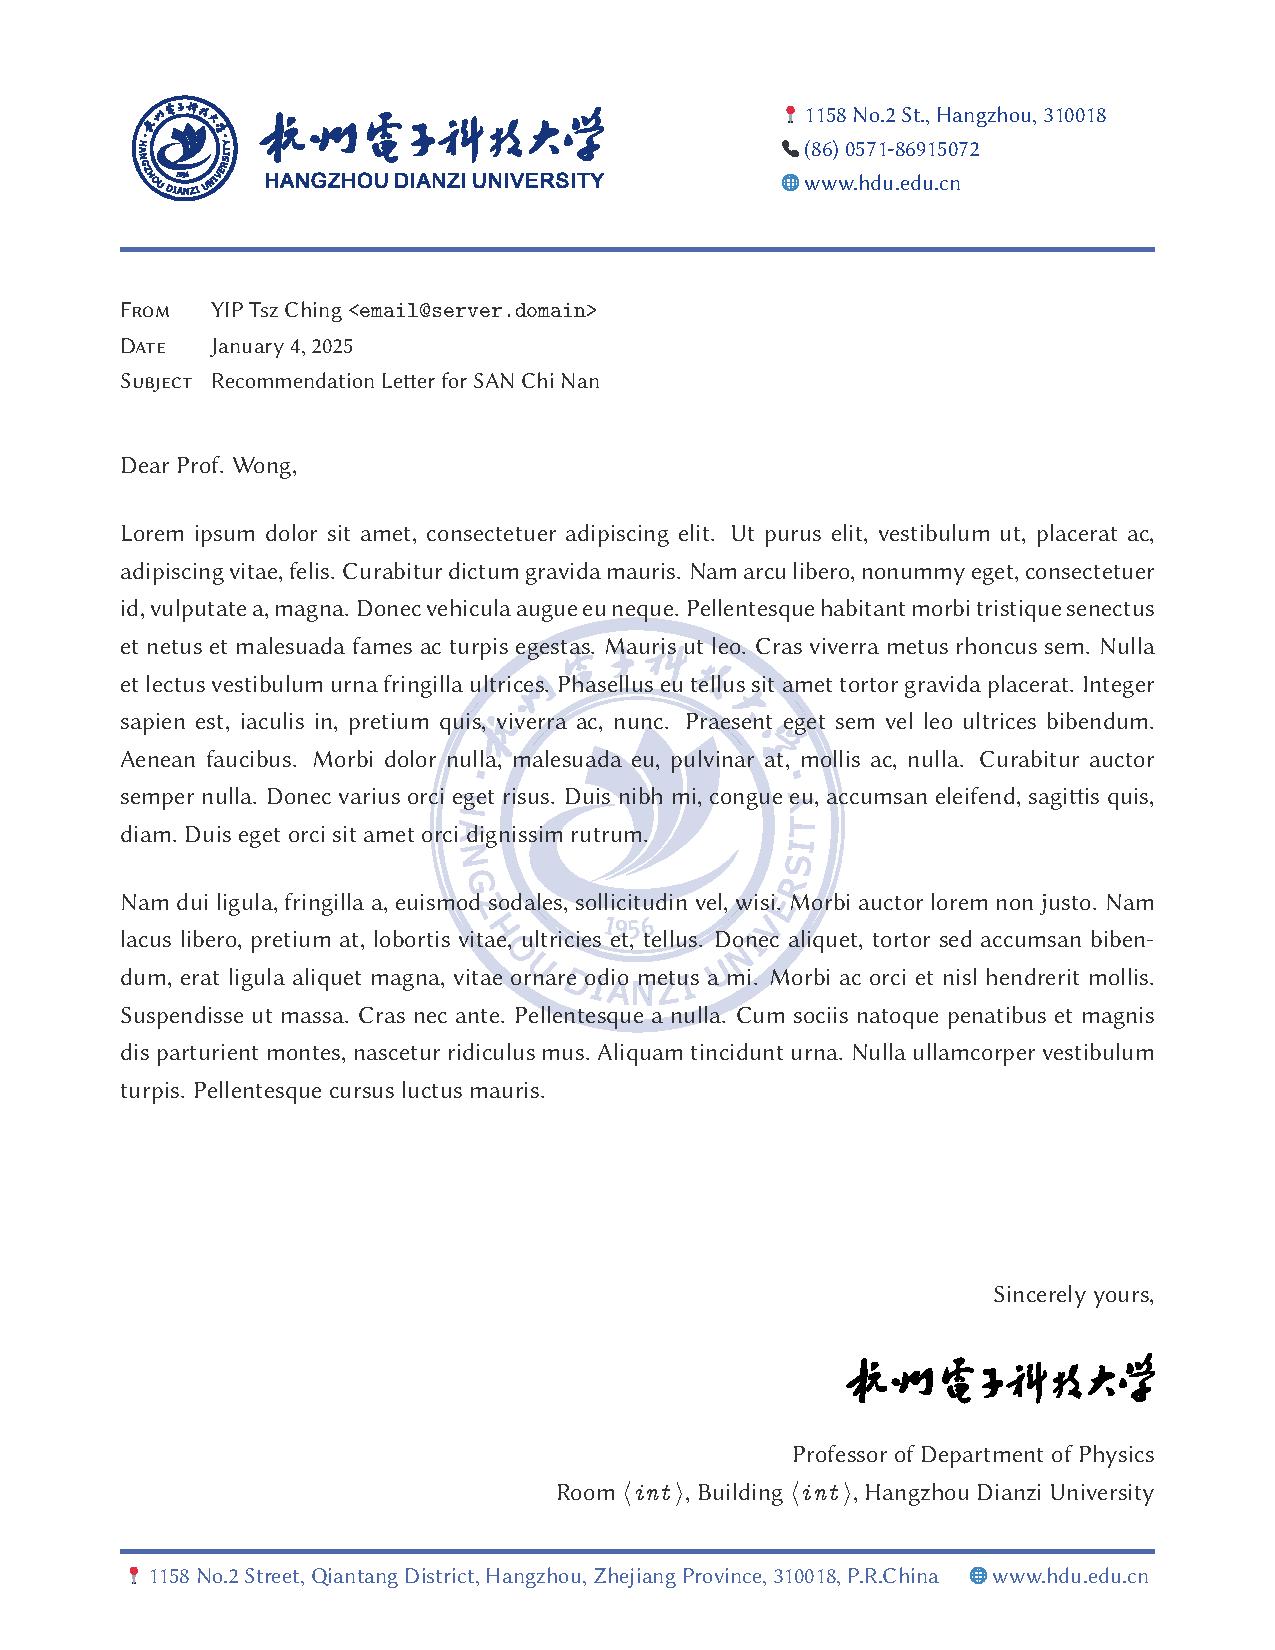
\includepdf [ pages = -, nup = 1x2, angle = -90, frame,
%               linktodoc, scale = 0.96, delta = 0in .25in
%             ] {hduthesis-stationery}
%
% \subsection{Beamer 主题}
%
% 本模板中存在独立的 Beamer 主题 "hdu",用于生成杭州电子科技大学风格的 Beamer 幻灯片.
% 由于本主题为杭州电子科技大学专属,所以该主题暂不开放更改主题色杭电蓝和Logo.
%
% 加载模块 \pkg{beamer},并进行文档信息设置,即以 "hdu" 为主题制作Beamer.
% 此模块无需 \pkg{agreed} 选项.
% \begin{quote}
%   |\documentclass [ mode = beamer ] { hduthesis }|
% \end{quote}
% 与学士 / 硕士学位论文文档信息设置类似,使用 \cs{DocInfo} 命令,
% 对信件主题、发件人、邮箱、日期和水印进行设置. 此时 \cs{DocInfo} 命令接受键
% \key*{title} \key*{subtitle} \key*{author} \key*{date} \key*{supervisor}
% \key*{reference}. 下页为生成Beamer的样例.
% \begin{verbatim}
%   \hduset
%     {
%       title      = Beamer Theme for Hangzhou Dianzi University
%                    Based on \LaTeX3,
%       subtitle   = hdu Undergraduate Thesis Proposal,
%       author     = SAN Chi Nan (C668668E0),
%       date       = {\today{} / Building 6, Room 321},
%       supervisor = Prof. YIP Tsz Ching,
%       bibsource  = reference.bib,
%     }
% \end{verbatim}
%
% \subsection{HDU 试卷解析模板}
%
% \begin{quote}
%   此模块开发中,敬请期待 |:-)|\quad [预计完成时间:14/03/2025].
%   \vspace{\baselineskip}
%   \begin{flushright}
%     |@myhsia|\\
%     Physics Department\\
%     Hangzhou Dianzi University
%   \end{flushright}
% \end{quote}
%
% 
\includepdf [ pages = -, nup = 2x4, frame, linktodoc,
%               scale = 0.96, delta = .25in .2in
%             ] {hduthesis-beamer.pdf}
%
% \begin{thebibliography}{99}
%   \bibitem{interface3} The \hologo{LaTeX} Project.
%   The \hologo{LaTeX3} Interfaces. CTAN: Released 2025-01-18.
%   \bibitem{ctex} \url{CTEX.ORG}. C\hologo{TeX} 宏集. 2022/07/14 v2.5.10.
%   \bibitem{clsguide} \hologo{LaTeX} Project Team.
%   LaTeX for package and class authors current version
%   \copyright{} Copyright 2023 -- 2024. 2024-09-15.
%   \bibitem{source2e} B. Johannes, C. David, J. Alan, L. Leslie L, M. Frank,
%   R. Chris, and S. Rainer.
%   \hologo{LaTeX} for package and class authors current version.
%   2024-11-01 Patch level 2.
%   \bibitem{l3styleguide} The \hologo{LaTeX} Project.
%   The \hologo{LaTeX3} kernel: style guide for code authors.
%   CTAN: Released 2025-01-18.
%   \bibitem{packages} Package \pkg{etoolbox}, \pkg{geometry}, \pkg{tocloft},
%   \pkg{fancyhdr}, etc.
%   \bibitem{hdubachelor} 杭州电子科技大学教务处.
%   \href{https://jwc.hdu.edu.cn/2022/0428/c4555a153813/page.htm}
%     {毕业设计(论文)的写作规范及格式要求}
%   \bibitem{hdumphil} 杭州电子科技大学研究生院.
%   \href{https://grs.hdu.edu.cn/2013/0507/c1730a51754/page.htm}
%     {杭州电子科技大学研究生学位论文格式统一要求(杭电研〔2012〕311号)}
% \end{thebibliography}
% \end{documentation}
% \restoregeometry \appendix
% \begin{implementation}
%
% \section{实现细节}
%
% \subsection{HDU 校徽 \& 校名 \& 校牌 \& 校训的实现}
%
% \subsubsection{原始素材预处理}
%
% 前往 \href{https://www.hdu.edu.cn/666/list.htm}{校情纵览/校标规范}
% 资源后,使用 Inkscape(或 Adobe Illustrator,Affinity Design,Vectornator 等)
% 分别将校徽、校名、校牌、校训导出 |.pdf| 格式. 校牌可能需要手动将校徽、校名手动拼接.
%
% \subsubsection{PDF 文件处理}
%
% 由于发行版 \hologo{TeX} Live 2024 及更早版本中的 |dvipdfmx| 程序在以指定透明度插入经
% Inkscape 导出的 |.pdf| 文件时存在透明度失效问题\footnote
% {感谢 \hologo{TeX} 专家 \href{https://www.zhihu.com/people/li-a-ling}
% {|@李阿玲|} 修复了这一 Bug (Commit: |fdefe61|).},
% 所以先使用 |Ghostscript| 程序修复 |.pdf| 文件
% \begin{quote}
%   "gs -o" \meta{input file}".pdf -sDEVICE=pdfwrite" \meta{output file}".pdf"
% \end{quote}
% 此时若使用 Text Editor 查看导出的 |.pdf| 文件,会发现里面存在许多无法识别的字符.
% 这时需要使用 mutool 工具对 |.pdf| 文件的内容流进行清理、消毒、压缩和数据转换. 命令如下
% \begin{quote}
%   "mutool clean -a -z -gggg" \meta{input file}".pdf" \meta{output file}".pdf"
% \end{quote}
%
% \subsubsection{素材打包}
%
% 由于每个 |.pdf| 文件均存在以 |%| 开头的代码
% \begin{verbatim}
%      %PDF-1.7
%      %µ¶
%      %%EOF
% \end{verbatim}
% 需更改 Docstrip 处理 |%| 行为:|%| 改为 |%%|,|%%| 改为 |%%%|,
% 并在 \file{hduthesis.ins} 添加
% \begin{quote}
%   "\let \MetaPrefix \perCent"
% \end{quote}
% 现可将处理结束后得到 ASCII 编码的 |.pdf| 文件,打包至 \file{hdu-graphics.dtx}.
%
% \subsection{\file{hduthesis.cls} 的实现}
%
%    \begin{macrocode}
%<@@=hdu>
%    \end{macrocode}
%
%    \begin{macrocode}
%<*class>
%    \end{macrocode}
%
%    \begin{macrocode}
\def \hduthesis@date {2025-03-07}
\def \hduthesis@version {1.0.0}
\def \hduthesis@maintainerid {myhsia}
%    \end{macrocode}
%
%    \begin{macrocode}
\ProvidesExplClass {hduthesis} {\hduthesis@date} {\hduthesis@version}
  {LaTeX Template Bundle for Hangzhou Dianzi University}
%    \end{macrocode}
%   兼容 \hologo{TeX} Live 2023 及之后的版本. 当对应命令不存在时,在已有命令基础上新增变体
%    \begin{macrocode}
\cs_if_exist:NF \seq_set_split:Nne
  { \cs_generate_variant:Nn \seq_set_split:Nnn { Nne } }
\cs_if_exist:NF \seq_set_split:Nee
  { \cs_generate_variant:Nn \seq_set_split:Nnn { Nee } }
\cs_if_exist:NF \tl_set:Ne
  { \cs_generate_variant:Nn \tl_set:Nn { Ne } }
\cs_if_exist:NF \tl_gset:Ne
  { \cs_generate_variant:Nn \tl_gset:Nn { Ne } }
%    \end{macrocode}
%   警告信息设置
%    \begin{macrocode}
\cs_new_protected:Npn \@@_msg_new:nn #1#2 
  { \msg_new:nnn { hduthesis } {#1} {#2} }
\cs_new_protected:Npn \@@_msg_error:nn #1#2
  { \msg_error:nnn { hduthesis } {#1} {#2} }
\cs_generate_variant:Nn \@@_msg_error:nn { nx }
\cs_new_protected:Npn \@@_msg_warning:nn #1#2
  { \msg_warning:nnn { hduthesis } {#1} {#2} }
\cs_generate_variant:Nn \@@_msg_warning:nn { nx }
\@@_msg_new:nn { not found module }
  { The ~ hduthesis ~ module ~ `#1' ~ not ~ found. }
\@@_msg_new:nn { unknown mode }
  { 
    Unknown ~ hduthesis ~ mode ~ `#1',~
    loading ~ mode ~ `thesis' ~ instead.
  }
\@@_msg_new:nn { Users Agreement }
  {
    \exp_not:n
      {
        编译受阻!~ 使用模板前请阅读用户手册中的「用户协议」
        \MessageBreak
        !模板作者 (@myhsia) 不对使用本模板产生的格式审查问题负责!
        \MessageBreak
        如果您同意协议,在全局选项中添加 `agreed' 即可解除本错误
        \MessageBreak
        欢迎您通过邮件 (myhsia@hdu.edu.cn) 或 GitHub 反馈意见
      }
  }
%    \end{macrocode}
% \begin{macro}{\@@_load_module:n, \@@_provide_module:n}
%   加载 / 提供 \cls{hduthesis} 的模块
%    \begin{macrocode}
\cs_new_protected_nopar:Npn \@@_load_module:n #1 
  {
    \clist_map_inline:nn {#1}
    {
      \file_if_exist_input:nF { hdu-##1.code.tex }
        { \@@_msg_error:nn { not found module } {##1} }
    }
  }
\cs_new_protected_nopar:Npn \@@_provide_module:n #1
  {
    \ProvidesExplFile{hdu-#1.code.tex}
      {\hduthesis@date}{\hduthesis@version}
      {hduThesiS ~ \text_titlecase:n {#1} ~ Module}
  }
%    \end{macrocode}
% \end{macro}
% \begin{variable}
%   {
%     \g_@@_agreement_bool, \g_@@_mode_tl,
%     \g_@@_math_font,      \g_@@_main_CJK_font,
%     \g_@@_sans_CJK_font,  \g_@@_mono_CJK_font
%   }
%   定义文档类全局选项的键.
%    \begin{macrocode}
\keys_define:nn { hduthesis / classoption }
  {
    agreed       .bool_set:N = \g_@@_agreement_bool,
      agreed     .initial:n  = false,
      agreed     .default:n  = true,
    mode         .tl_set:N   = \g_@@_mode_tl,
    math-font    .tl_set:N   = \g_@@_math_font,
    CJKmain-font .tl_set:N   = \g_@@_main_CJK_font,
    CJKsans-font .tl_set:N   = \g_@@_sans_CJK_font,
    CJKmono-font .tl_set:N   = \g_@@_mono_CJK_font,
    unknown      .code:n     = \@@_unknown_option:n {#1},
  }
%    \end{macrocode}
% \end{variable}
% \begin{macro}{\@@_unknown_option:n}
% \begin{variable}{\g_@@_base_options_clist}
%   用于接收其他对此文档类未知选项.
%    \begin{macrocode}
\clist_new:N \g_@@_base_options_clist
%    \end{macrocode}
% \end{variable}
%   处理未知选项:移交基本文档类处理.
%    \begin{macrocode}
\cs_new_protected_nopar:Npn \@@_unknown_option:n #1
  {
    \tl_if_empty:nTF { #1 }
      {
        \clist_gput_right:NV
          \g_@@_base_options_clist \l_keys_key_str
      }
      {
        \exp_args:NNx
        \clist_gput_right:Nn \g_@@_base_options_clist
          { \l_keys_key_str = \exp_not:n {#1} }
      }
  }
%    \end{macrocode}
% \end{macro}
%   处理接收到的全局选项.
%    \begin{macrocode}
\ProcessKeyOptions [ hduthesis / classoption ]
%    \end{macrocode}
%   遇到未知模块时返回警告信息.
%    \begin{macrocode}
\bool_lazy_all:nT
  {
    { !\str_if_empty_p:N \g_@@_mode_tl }
    { !\str_if_eq_p:ee { \g_@@_mode_tl } { thesis } }
    { !\str_if_eq_p:ee { \g_@@_mode_tl } { beamer } }
    { !\str_if_eq_p:ee { \g_@@_mode_tl } { stationery } }
    { !\str_if_eq_p:ee { \g_@@_mode_tl } { exam } }
    { !\str_if_eq_p:ee { \g_@@_mode_tl } { l3doc } }
  }
  { \@@_msg_warning:nx { unknown mode } { \g_@@_mode_tl } }
%    \end{macrocode}
%   加载 \module{beamer} 模块.
%    \begin{macrocode}
\str_if_eq:eeT { \g_@@_mode_tl } { beamer }
  {
    \PassOptionsToClass { aspectratio = 2013 } { beamer }
    \exp_args:NNV
    \LoadClass [ \g_@@_base_options_clist ] { beamer }
    \usetheme{hdu}
    \endinput
  }
%    \end{macrocode}
%   加载 \module{stationery} 模块.
%    \begin{macrocode}
\str_if_eq:eeT { \g_@@_mode_tl } { stationery }
  {
    \PassOptionsToClass { 12pt } { letter }
    \exp_args:NNV
    \LoadClass [ \g_@@_base_options_clist ] { letter }
    \@@_load_module:n { stationery }
    \endinput
  }
%    \end{macrocode}
%   加载 \module{exam} 模块.
%    \begin{macrocode}
\str_if_eq:eeT { \g_@@_mode_tl } { exam }
  {
    \exp_args:NNV
    \LoadClass [ \g_@@_base_options_clist ] { article }
    \@@_load_module:n { exam }
    \endinput
  }
%    \end{macrocode}
%   加载 \module{l3doc} 模块.
%    \begin{macrocode}
\str_if_eq:eeT { \g_@@_mode_tl } { l3doc }
  {
    \PassOptionsToClass { 11pt, letterpaper, kernel } { l3doc }
    \RequirePackage{minted}
    \exp_args:NNV
    \LoadClass [ \g_@@_base_options_clist ] { l3doc }
    \@@_load_module:n { l3doc }
    \endinput
  }
%    \end{macrocode}
%   其余情况下,默认加载 \module{thesis} 模块,并根据所输入的学号位数加载不同配置.
%   未确认用户协议时,返回错误信息.
%    \begin{macrocode}
\bool_lazy_any:nT
  {
    { \str_if_eq_p:ee { \g_@@_mode_tl } { thesis } }
    { !\str_if_eq_p:ee { \g_@@_mode_tl } { beamer } }
    { !\str_if_eq_p:ee { \g_@@_mode_tl } { stationery } }
    { !\str_if_eq_p:ee { \g_@@_mode_tl } { exam } }
    { !\str_if_eq_p:ee { \g_@@_mode_tl } { l3doc } }
  }
  {
    \PassOptionsToClass { a4paper, zihao = -4 } { ctexrep }
    \PassOptionsToPackage { quiet, no-math } { xeCJK }
    \exp_args:NNV
    \LoadClass [ \g_@@_base_options_clist ] { ctexrep }
    \bool_if:NTF \g_@@_agreement_bool
      {
        \RequirePackage{hyperref}
        \pdfstringdefDisableCommands
          {
            \def \cite#1 {<#1>}
            \def \hologoRobust#1 {<#1>}
          }
        \AtBeginDocument
          {
            \hypersetup
              { hidelinks, pdfproducer = hduThesiS ~ by ~ Mingyu ~ Xia }
          }
      } { \@@_msg_error:nn { Users Agreement } { Unconfirmed } }
    \@@_load_module:n { typeset }
    \@@_load_module:n { layout }
    \cs_new_protected:Nn \@@_docinfo_degree_if_aux:
      {
        \int_compare:nNnTF
          { \tl_count:N \l_@@_set_stdntid_tl } = { 8 }
          { \@@_load_module:n { bc.config } }
          { \@@_load_module:n { pg.config } }
      }
    \endinput
  }
%    \end{macrocode}
%
%    \begin{macrocode}
%</class>
%    \end{macrocode}
%
% \subsection{\module{typeset} 模块的实现}
%
%    \begin{macrocode}
%<*typeset>
%    \end{macrocode}
%
%    \begin{macrocode}
\@@_provide_module:n {typeset}
%    \end{macrocode}
%
%    \begin{macrocode}
\RequirePackage { circuitikz, pgfplots, listings, hologo,
                  lipsum, zhlipsum, booktabs, multicol }
\pgfplotsset { compat = newest }
\hologoFontSetup { general = \sffamily }
%    \end{macrocode}
%   插图相对路径设置.
%    \begin{macrocode}
\graphicspath
  {
    {./figure/}{./figures/}{./image/}{./images/}
    {./graphics/}{./graphic/}{./pictures/}{./picture/}
  }
%    \end{macrocode}
%   设置行距倍数和缩进.
%    \begin{macrocode}
\linespread{1.39}
\dim_set:Nn \parindent { 2\ccwd }
%    \end{macrocode}
% \begin{macro}{\@@_font_semilarge:, \@@_font_semiLarge:}
%   两种新字体尺寸设置.
%    \begin{macrocode}
\cs_new_protected:Nn \@@_font_semilarge:
  { \@setfontsize \@@_font_semilarge:{14}{16.5} }
\cs_new_protected:Nn \@@_font_semiLarge:
  { \@setfontsize \@@_font_semiLarge:{16.5}{17.5} }
%    \end{macrocode}
% \end{macro}
%   设置西文字体
%    \begin{macrocode}
\setmainfont{texgyretermes}
  [
    Extension      = .otf,         UprightFont = *-regular,
    BoldFont       = *-bold,       ItalicFont  = *-italic,
    BoldItalicFont = *-bolditalic
  ]
\setsansfont{texgyreheros}
  [
    Extension      = .otf,         BoldItalicFont = *-bolditalic,
    UprightFont    = *-regular,    BoldFont       = *-bold,
    ItalicFont     = *-italic,     Scale          = .9
  ]
%    \end{macrocode}
%   公式排版必要宏包加载,行间公式前后间距设置.
%    \begin{macrocode}
\RequirePackage { mathtools,  amssymb, cancel,  fixdif,
                  derivative, siunitx, physics2 }
\usephysicsmodule { ab, braket, op.legacy, bm-um.legacy }
\RequirePackage
  [ warnings-off = { mathtools-colon, mathtools-overbracket }
  ] {unicode-math}
\AtBeginDocument
  {
    \dim_set:Nn \abovedisplayskip {3pt}
    \dim_set:Nn \belowdisplayskip {3pt}
  }
%    \end{macrocode}
%   数学字体、中文字体设置.
%    \begin{macrocode}
\tl_if_empty:NF \g_@@_math_font
  { \setmathfont { \g_@@_math_font } }
\tl_if_empty:NF \g_@@_main_CJK_font
  { \exp_last_unbraced:No \setCJKmainfont \g_@@_main_CJK_font }
\tl_if_empty:NF \g_@@_sans_CJK_font
  { \exp_last_unbraced:No \setCJKsansfont \g_@@_sans_CJK_font }
\tl_if_empty:NF \g_@@_mono_CJK_font
  { \exp_last_unbraced:No \setCJKmonofont \g_@@_mono_CJK_font }
%    \end{macrocode}
%
%    \begin{macrocode}
%</typeset>
%    \end{macrocode}
%
% \subsection{\module{layout} 模块的实现}
%
%    \begin{macrocode}
%<*layout>
%    \end{macrocode}
%
%    \begin{macrocode}
\@@_provide_module:n {layout}
%    \end{macrocode}
%   页面样式、编号、列表设置.
%    \begin{macrocode}
\RequirePackage { geometry, array, setspace,
                  fancyhdr, enumitem, cleveref }
\RequirePackage
  [ skip = 1.75ex, labelsep = quad, font = small ]{caption}
\fancyhf{}
\pagestyle{fancy}
\renewcommand*\headrulewidth {.8pt}
\renewcommand*\thefigure {\arabic{chapter}-\arabic{figure}}
\renewcommand*\thetable {\arabic{chapter}-\arabic{table}}
\renewcommand*\theequation {\arabic{chapter}-\arabic{equation}}
\AddToHook{env/figure/after}{\vspace*{-2.3ex}}
\AddToHook{env/table/after}{\vskip-1.9ex}
\setlist[enumerate,1]
  {
    label = (\,\arabic*\,), itemindent = 4em, leftmargin = 0em,
    labelsep = 1ex, topsep = 0pt, itemsep = 0pt, partopsep = 0pt,
    parsep = 0em, listparindent = 2\ccwd
  }
\crefformat{figure}{图#2#1#3}
\crefformat{table}{表#2#1#3}
%    \end{macrocode}
% \begin{macro}{\@@_cover_spread_box:nn, \@@_cover_center_box:nn}
%   分散对齐盒子与\ulem{下划线居中对齐盒子}.
%   \footnote{由 \url{tex.stackexchange.com} 论坛上 |@egreg| 提供接口.}
%    \begin{macrocode}
\cs_new_protected:Npn \@@_cover_spread_box:nn #1#2
  {
    \mode_leave_vertical:
    \hbox_to_wd:nn {#1}
      { \exp_args:Nee \tl_map_inline:nn {#2} { ##1 \hfil } \unskip }
  }
\cs_new_protected:Npn \@@_cover_center_box:nn #1#2
  {
    \mode_leave_vertical:
    \dim_set:Nn \l_tmpa_dim {#1}
    \global\setbox1 = \box\voidb@x
    \group_begin:
    \setbox0 = \vbox
      {
        \dim_set:Nn \hsize {#1}\relax
        \dim_set:Nn \parindent {0pt}
        \skip_set:Nn \leftskip {0pt plus 1fil}
        \skip_set:Nn \rightskip {0pt plus -1fil}
        \skip_set:Nn \parfillskip {0pt plus 2fil}
        #2 \par
        \loop
        \setbox2 = \lastbox
        \unless\ifvoid2
          \global\setbox1 = \vtop
            { \hbox to\hsize{\strut\unhbox2}
              \vskip-4pt \hrule height .5pt
              \vskip9.6pt \unvbox1
            }
          \unskip\unpenalty
        \repeat
      }
    \group_end:
    \box1
  }
%    \end{macrocode}
% \end{macro}
% \begin{macro}{\@@_process_array:NnnN}
%   拆分 \cs{hduset} 部分键值输入二维数组.
%    \begin{macrocode}
\cs_new_protected_nopar:Npn \@@_process_array:NnnN #1#2#3#4
  {
    \seq_set_split:Nee \l_@@_process_array_seq { / } {#1}
    \seq_set_split:Nee \l_@@_process_array_row_seq { \c_colon_str }
      { \seq_item:Nn \l_@@_process_array_seq {#2} }
    \tl_if_eq:nnTF {#3} {:}
      {
        \tl_gset:Ne #4
          { \seq_use:Nn \l_@@_process_array_row_seq {} }
      }
      {
        \tl_gset:Ne #4
          { \seq_item:Nn \l_@@_process_array_row_seq {#3} }
      }
    \seq_clear:N \l_@@_process_array_seq
    \seq_clear:N \l_@@_process_array_row_seq
  }
%    \end{macrocode}
% \end{macro}
% \begin{variable}{\g_@@_month_clist}
%   存储英文月份表达.
%    \begin{macrocode}
\clist_set:Nn \g_@@_month_clist
  {
    January, February,  March,     April,   May,      June,
    July,    August,    September, October, November, December
  }
%    \end{macrocode}
% \end{variable}
% \begin{variable}
%   {
%     \l_@@_set_title_tl,      \l_@@_set_department_tl,
%     \l_@@_set_major_tl,      \l_@@_set_class_tl,
%     \l_@@_set_stdntid_tl,    \l_@@_set_author_tl,
%     \l_@@_set_supervisor_tl, \l_@@_set_bibsource_tl
%   }
%   模式 \module{thesis} 下 \cs{hduset} 接口键值的定义.
%    \begin{macrocode}
\keys_define:nn { thesis / hduset }
  {
    title      .clist_set:N = \l_@@_set_title_tl,
    department .tl_set:N    = \l_@@_set_department_tl,
    major      .tl_set:N    = \l_@@_set_major_tl,
    class      .tl_set:N    = \l_@@_set_class_tl,
    stdntid    .tl_set:N    = \l_@@_set_stdntid_tl,
    author     .clist_set:N = \l_@@_set_author_tl,
    supervisor .tl_set:N    = \l_@@_set_supervisor_tl,
    bibsource  .tl_set:N    = \l_@@_set_bibsource_tl,
  }
%    \end{macrocode}
% \end{variable}
% \begin{macro}{\hduset}
%   模式 \module{thesis} 下设置文档信息.
%    \begin{macrocode}
\NewDocumentCommand \hduset { m }
  {
    \keys_set:nn { thesis / hduset } {#1}
    \@@_docinfo_process_aux:  
    \@@_docinfo_degree_if_aux:  
  }
%    \end{macrocode}
% \end{macro}
% \begin{macro}{\@@_docinfo_process_aux:}
%   模式 \module{thesis} 下 \cs{hduset} 的辅助命令:拆分数组 / 设置参考文献.
%    \begin{macrocode}
\cs_set_protected_nopar:Nn \@@_docinfo_process_aux:
  {
    \@@_process_array:NnnN \l_@@_set_title_tl {1} {:} \@title
    \@@_process_array:NnnN \l_@@_set_title_tl {2} {:}
      \l_@@_set_entitle_tl
    \@@_process_array:NnnN \l_@@_set_author_tl {1} {:} \@author
    \@@_process_array:NnnN \l_@@_set_author_tl {2} {:}
      \l_@@_set_enauthor_tl
    \@@_process_array:NnnN \l_@@_set_supervisor_tl {1} {1}
      \l_@@_set_cnrole_tl
    \@@_process_array:NnnN \l_@@_set_supervisor_tl {1} {2}
      \l_@@_set_cnsupervisor_tl
    \@@_process_array:NnnN \l_@@_set_supervisor_tl {2} {1}
      \l_@@_set_enrole_tl
    \@@_process_array:NnnN \l_@@_set_supervisor_tl {2} {2}
      \l_@@_set_ensupervisor_tl
    \bool_if:NF \g_@@_agreement_bool
      { \tl_clear:N \l_@@_set_bibsource_tl }
    \tl_if_empty:NTF \l_@@_set_bibsource_tl
      {
        \newcommand*\printbibliography{\chapter*{参考文献}}
        \newcounter {citecount}
        \renewcommand*\cite[1]
          {
            \refstepcounter{citecount}
            \textsuperscript{[\thecitecount]}
          }
      }
      {
        \RequirePackage[sort&compress]{gbt7714}
        \bibliographystyle{gbt7714-numerical}
        \dim_set:Nn \bibsep {.35ex}
        \newcommand*\printbibliography
          {
            \bibliography { \l_@@_set_bibsource_tl }
            \addcontentsline{toc}{chapter}{参考文献}
          }
      }
  }
%    \end{macrocode}
% \end{macro}
% \begin{macro}{\@@_commitment_sign:N}
%   插入签名图片.
%    \begin{macrocode}
\cs_new_protected:Npn \@@_commitment_sign:N #1
  {
    \leavevmode@ifvmode
    \lower \dimexpr \f@size\p@ * 9/16
    \hbox
      {
        \includegraphics
          [ height = { \fp_eval:n { 2*\f@size }\p@ } ] {#1}
      }
  }
%    \end{macrocode}
% \end{macro}
% \begin{macro}{\@@_sign_process_aux:nnn}
%   处理承诺书签名数组的辅助命令. 签名文件名需要展开后存入
%   \cs{l_@@_sign_figure_tl} 中.
%    \begin{macrocode}
\cs_new_protected_nopar:Npn \@@_sign_process_aux:nnn #1#2#3
  {
    \clist_set:Nn \l_@@_sign_process_clist {#1}
    \seq_set_split:Nne \l_@@_sign_figure_seq {/}
      { \clist_item:Nn \l_@@_sign_process_clist {#2} }
    \int_compare:nNnTF {#3} = {0}
      {
        \tl_set:Ne \l_@@_sign_figure_tl
          { \seq_item:Nn \l_@@_sign_figure_seq { #3 + 1 } }
        \seq_clear:N \l_@@_sign_figure_seq
      }
      {
        \seq_set_split:Nne \l_@@_sign_date_seq {-}
          { \seq_item:Nn \l_@@_sign_figure_seq {2} }
        \seq_item:Nn \l_@@_sign_date_seq {#3}
        \seq_clear:N \l_@@_sign_date_seq
      }
    \clist_clear:N \l_@@_sign_process_clist
  }
%    \end{macrocode}
% \end{macro}
%
%    \begin{macrocode}
%</layout>
%    \end{macrocode}
%
% \subsection{\module{bc.config} 模块的实现}
%
%    \begin{macrocode}
%<*bc.config>
%    \end{macrocode}
%
%    \begin{macrocode}
\ExplSyntaxOn \makeatletter
%    \end{macrocode}
%
%    \begin{macrocode}
\@@_provide_module:n {bc.config}
%    \end{macrocode}
%   设置页面布局、页眉、目录页码格式.
%    \begin{macrocode}
\geometry { top     = 3.25cm, bottom     = 2.4cm,
            left    = 4cm,    right      = 2cm,
            headsep = .72cm,  headheight = 15pt }
\fancyhead[C]
  {
    \raisebox { .12ex }
      { \small 杭州电子科技大学 \l_@@_set_entitle_tl }
  }
\hook_gput_code:nnn {cmd/tableofcontents/before} { . }
  {
    \clearpage 
    \pagenumbering{Roman} \cfoot{\small \thepage}
  }
\hook_gput_code:nnn { cmd/tableofcontents/after } { . }
  {
    \thispagestyle{fancy} \clearpage
    \pagenumbering{arabic} \cfoot{}
  }
%    \end{macrocode}
% \begin{macro}{\maketitle}
%   重新定义封面布局.
%    \begin{macrocode}
\RenewDocumentCommand \maketitle {}
  {
    \newgeometry { margin = 3cm }
    \titlepage \@@_maketitle_bc_auxi: \endtitlepage
    \restoregeometry
  }
%    \end{macrocode}
% \end{macro}
% \begin{variable}{\l_@@_grade_int}
%   存储毕业年份. 根据当前月份判断.
%    \begin{macrocode}
\int_new:N \l_@@_grade_int
\int_set:Nn \l_@@_grade_int
  {
    \int_compare:nNnTF { \c_sys_month_int } < 9
      { \c_sys_year_int } { \int_eval:n { \c_sys_year_int + 1 } }
  }
%    \end{macrocode}
% \end{variable}
% \begin{macro}{\@@_maketitle_bc_auxi:}
%   \cs{maketitle} 的辅助命令.
%    \begin{macrocode}
\cs_new_protected_nopar:Nn \@@_maketitle_bc_auxi:
  {
    \begin{center}
      \vspace*{14\p@}
      
\includegraphics[ width = .64\linewidth ]{hdutitle}
      \par \vspace*{36\p@}
      \scalebox{2.75}
      {
        \textbf
          {
            \@@_cover_spread_box:nn
              { .205\paperwidth } { \l_@@_set_entitle_tl }
          }
      }
      \par \vspace*{1.5\baselineskip}
      { \LARGE (\int_use:N \l_@@_grade_int \bfseries 届) }
      \par \vspace*{3.0\baselineskip}
      \begin{tabular}
        {
          >{\large\bfseries}p{5.5\ccwd}@{}
          >{\large\centering\arraybackslash\kaishu}p{.65\linewidth}@{}
        }
        \@@_cover_spread_box:nn { 4\ccwd } { 题目 } &
        \@@_cover_center_box:nn { .95\linewidth }
          { \@title }\\[5.2ex]
        \@@_cover_spread_box:nn { 4\ccwd } { 学院 } &
        \@@_cover_center_box:nn { .95\linewidth }
          { \l_@@_set_department_tl }\\[5.2ex]
        \@@_cover_spread_box:nn { 4\ccwd } { 专业 } &
        \@@_cover_center_box:nn { .95\linewidth }
          { \l_@@_set_major_tl }\\[5.2ex]
        \@@_cover_spread_box:nn { 4\ccwd } { 班级 } &
        \@@_cover_center_box:nn { .95\linewidth }
          { \l_@@_set_class_tl }\\[5.2ex]
        \@@_cover_spread_box:nn { 4\ccwd } { 学号 } &
        \@@_cover_center_box:nn { .95\linewidth }
          { \l_@@_set_stdntid_tl }\\[5.2ex]
        \@@_cover_spread_box:nn { 4\ccwd } { 学生姓名 } &
        \@@_cover_center_box:nn { .95\linewidth }
          { \@author }\\[5.2ex]
        \@@_cover_spread_box:nn { 4\ccwd } { 指导教师 } &
        \@@_cover_center_box:nn { .95\linewidth }
          {
            \l_@@_set_cnsupervisor_tl \quad
            \l_@@_set_cnrole_tl
          }\\[5.2ex]
        \@@_cover_spread_box:nn { 4\ccwd } { 完成日期 } &
        \@@_cover_center_box:nn { .95\linewidth }
          {
            \textsf{\int_use:N \c_sys_year_int} 年
            \textsf{\int_use:N \c_sys_month_int} 月
          }
      \end{tabular}
    \end{center}
  }
%    \end{macrocode}
% \end{macro}
% \begin{macro}{\commitment}
%   生成承诺书
%    \begin{macrocode}
\NewDocumentCommand \commitment { O{} }
  {
    \newgeometry{ margin = 3cm }
    \titlepage
      \@@_commitment_bc_aux:n {#1}
    \endtitlepage
    \restoregeometry
  }
%    \end{macrocode}
% \end{macro}
% \begin{macro}{\@@_commitment_bc_aux:n}
%   \cs{commitment} 的辅助命令.
%    \begin{macrocode}
\cs_new_protected_nopar:Npn \@@_commitment_bc_aux:n #1
  {
    \vspace*{65\p@}
    \begin{center}
      \@beginparpenalty \@lowpenalty
      \Large \textsf
        { \bfseries \@@_cover_spread_box:nn { 6\ccwd }{ 诚信承诺 } }
      \@endparpenalty \@M
    \end{center}
    \vspace*{.4\baselineskip} \par
    \linespread{2.1}
      {
        \@@_font_semilarge:
        我谨在此承诺:本人所写的毕业论文《\@title 》均系本人独立完成,
        没有抄袭行为,凡涉及其他作者的观点和材料,均作了注释,若有不实,
        后果由本人承担。
        \par\vspace*{\baselineskip} \bfseries\sffamily
        \hskip.48\linewidth 承诺人(签名):
        \@@_sign_process_aux:nnn {#1} { 1 } { 0 }
        \tl_if_empty:NF \l_@@_sign_figure_tl
          {
            \@@_commitment_sign:N
              \l_@@_sign_figure_tl
            \tl_clear:N \l_@@_sign_figure_tl
          }
        \par \vspace*{.5\baselineskip}
        \hskip \dim_eval:n { .48\linewidth - 1em }
        \makebox [ 3em ]
          { \@@_sign_process_aux:nnn {#1} { 1 } { 1 } } 年
        \makebox [ 2em ]
          { \@@_sign_process_aux:nnn {#1} { 1 } { 2 } } 月
        \makebox [ 2em ]
          { \@@_sign_process_aux:nnn {#1} { 1 } { 3 } } 日
      }
  }
%    \end{macrocode}
% \end{macro}
% \DescribeEnv{abstract}
%   重新定义摘要环境,加入中英文判断.
%    \begin{macrocode}
\RenewDocumentEnvironment {abstract} { O{en} }
  {
    \str_if_eq:nnT {#1} {en}
      {
        \tl_set:Nn \l_@@_keywords_name_tl {Keywords:~}
        \tl_set:Nn \l_@@_keywords_sep_tl {;~}
        \@beginparpenalty \@lowpenalty
        \chapter*{\normalfont\bfseries ABSTRACT}
      }
    \str_if_eq:nnT {#1} {cn}
      {
        \tl_set:Nn \l_@@_keywords_name_tl {\textsf{关键词:}}
        \tl_set:Nn \l_@@_keywords_sep_tl {;}
        \@beginparpenalty \@lowpenalty
        \chapter*{摘\qquad 要}
      }
  }
  {
    \tl_clear:N \l_@@_abstract_title_tl
    \cfoot{} \clearpage
  }
%    \end{macrocode}
% \begin{variable}{\l_@@_keywords_clist}
%   存储关键词列表.
%    \begin{macrocode}
\clist_new:N \l_@@_keywords_clist
%    \end{macrocode}
% \end{variable}
% \begin{macro}{\keywords}
%   重新定义 \cs{keywords} 命令,关键词样式会根据 \env{abstract} 所选语言自动变化.  
%    \begin{macrocode}
\NewDocumentCommand \keywords { m }
  {
    \par \vspace*{\baselineskip}
    \noindent\textbf{\l_@@_keywords_name_tl}
    \clist_set:Nn \l_@@_keywords_clist {#1}
    \clist_use:Nn \l_@@_keywords_clist {\l_@@_keywords_sep_tl}
  }
%    \end{macrocode}
% \end{macro}
%   设置目录样式.
%    \begin{macrocode}
\RequirePackage{tocloft}
\renewcommand \contentsname {\hfill 目 \qquad 录 \hfill}
\renewcommand* \cfttoctitlefont {\sffamily\@@_font_semiLarge:}
\dim_set:Nn \cftbeforetoctitleskip {3pt}
\dim_set:Nn \cftaftertoctitleskip {24pt}
\dim_set:Nn \cftbeforechapskip {1pt}
\dim_set:Nn \cftbeforesecskip {-.2pt}
\patchcmd { \@dottedtocline }
  {
    \leaders
    \hbox { $\m@th\mkern \@dotsep mu\hbox{.}\mkern \@dotsep mu$ }
  }
  {
    \kern 4pt \leaders
    \hbox { $\m@th\mkern .4 mu\hbox{-}\mkern .4 mu$ }
  } {}{}
\renewcommand* \l@chapter {\@dottedtocline{1}{0em}{1.6em}}
\renewcommand* \l@section {\@dottedtocline{1}{2.3em}{2.1em}}
\renewcommand* \@dotsep {1.7}
\renewcommand* \@pnumwidth {2.5ex}
\renewcommand* \cftchapfont {\normalfont}
\setcounter{tocdepth}{1}
%    \end{macrocode}
%   使用 \cs{ctexset} 提供的接口设置章节样式.
%    \begin{macrocode}
\ctexset
  {
    chapter    =
      {
        fixskip = true, name = {},  beforeskip = 21pt,
        format+ = \sffamily \large, afterskip  = 34pt,
        number  = \arabic{chapter}, pagestyle  = fancy,
      },
    section    =
      {
        beforeskip = 1.25ex, fixskip = true,
        afterskip  = 1.5ex,  format  = \sffamily \@@_font_semilarge:
      },
    subsection =
      {
        beforeskip = 1.25ex, fixskip = true,
        afterskip  = 1.5ex,  format  = \sffamily
      }
  }
%    \end{macrocode}
%
%    \begin{macrocode}
\makeatother \ExplSyntaxOff
%    \end{macrocode}
%
%    \begin{macrocode}
%</bc.config>
%    \end{macrocode}
%
% \subsection{\module{pg.config} 模块的实现}
%
%    \begin{macrocode}
%<*pg.config>
%    \end{macrocode}
%
%    \begin{macrocode}
\ExplSyntaxOn \makeatletter
%    \end{macrocode}
%
%    \begin{macrocode}
\@@_provide_module:n {pg.config}
%    \end{macrocode}
%   设置页面布局、页眉、目录页码格式.
%    \begin{macrocode}
\geometry { top = 2.8cm, bottom = 3.2cm, left = 3.2cm, right = 3.2cm,
            headheight = 15pt, headsep = .72cm, footskip = 1.5cm }
\fancyhead[C]
  { \raisebox { .12ex } { \small 杭州电子科技大学硕士学位论文 } }
\hook_gput_code:nnn { cmd/tableofcontents/after } { . }
  {
    \clearpage
    \pagenumbering{arabic}
    \cfoot{\small \thepage}
  }
%    \end{macrocode}
%   重新定义封面布局.
%    \begin{macrocode}
\RenewDocumentCommand \maketitle {}
  {
    \newgeometry{margin = 2.75cm}
    \begin{titlepage}
      \@@_maketitle_pg_auxi:
    \end{titlepage}
    \titlepage
      \@@_maketitle_pg_auxii:
    \endtitlepage
    \titlepage
      \@@_maketitle_pg_auxiii:
    \endtitlepage
    \restoregeometry
    \pagenumbering{Roman}
    \cfoot {\small \thepage}
  }
%    \end{macrocode}
% \begin{macro}
%   {\@@_maketitle_pg_auxi:, \@@_maketitle_pg_auxii:, \@@_maketitle_pg_auxiii:}
%   \cs{maketitle} 的辅助命令:封面设置、中文扉页设置、英文扉页设置.
%    \begin{macrocode}
\cs_new_protected_nopar:Nn \@@_maketitle_pg_auxi:
  {
    \begin{center}
      \null
      
\includegraphics[height = 2.35cm]{hdutitle}
      \par \vspace*{40\p@}
        {
          \LARGE
          \@@_cover_spread_box:nn {.575\linewidth} {硕士学位论文}
        }
      \par\vspace*{100\p@}
      \@@_font_semiLarge: 题 \qquad 目:
      \@@_cover_center_box:nn { .75\linewidth } { \kaishu \@title }
      \vspace*{24\p@}\par
      \begin{tabular}
        {
          >{ \@@_font_semiLarge: \centering \arraybackslash }
            p{4\ccwd}@{}
          >{ \@@_font_semiLarge: \centering \arraybackslash \kaishu }
            p{.65\linewidth}@{}
        }
        \@@_cover_spread_box:nn { 4\ccwd } { 研究生 } &
        \@@_cover_center_box:nn { .96\linewidth } { \@author }\\
        \@@_cover_spread_box:nn { 4\ccwd } { 专业 } &
        \@@_cover_center_box:nn { .96\linewidth }
          { \l_@@_set_major_tl }\\
        \@@_cover_spread_box:nn { 4\ccwd } { 指导教师 } &
        \@@_cover_center_box:nn { .96\linewidth }
          {
            \l_@@_set_cnsupervisor_tl \qquad \l_@@_set_cnrole_tl 
          }\\[13.5ex]
        \@@_font_semilarge: 完成日期 &
        \@@_cover_center_box:nn { .96\linewidth }
          {
            \@@_font_semilarge:
            \textsf { \int_use:N \c_sys_year_int } 年
            \textsf { \int_use:N \c_sys_month_int } 月
          }
      \end{tabular}
    \end{center}
  }
\cs_new_protected_nopar:Nn \@@_maketitle_pg_auxii:
  {
    \begin{center}
      \vspace*{25\p@}
        { \LARGE 杭州电子科技大学硕士学位论文 }
        \vspace*{140\p@} \par
        \begin{spacing}{1.15}
          \huge\textsf{ \@title }
        \end{spacing}
        \vspace*{128\p@} \par
        \begin{tabular}
          {
            >{ \@@_font_semiLarge: } p{6.25\ccwd}
            >{ \@@_font_semiLarge: \kaishu } l
          }
          \@@_cover_spread_box:nn { 4\ccwd } { 研究生 }:& 
          \@@_cover_spread_box:nn { 4\ccwd } { \@author }\\[2ex]
          \@@_cover_spread_box:nn { 4\ccwd } { 指导教师 }:&
          \@@_cover_spread_box:nn { 4\ccwd }
            { \l_@@_set_cnsupervisor_tl }
          \hskip 1.5em \l_@@_set_cnrole_tl
        \end{tabular}
        \par \vspace{60\p@} \@@_font_semilarge:
        \textsf { \int_use:N \c_sys_year_int } \kaishu 年
        \textsf { \int_use:N \c_sys_month_int } \kaishu 月
    \end{center}
  }
\cs_new_protected_nopar:Nn \@@_maketitle_pg_auxiii:
  {
    \begin{center}
      \vspace*{16\p@}
      {
        \bfseries \@@_font_semilarge:
        Dissertation ~ Submitted ~ to ~
        Hangzhou ~ Dianzi ~ University\\[.8ex]
        for ~ the ~ Degree ~ of ~ Master
      }
      \vspace*{120\p@} \par
      \begin{spacing}{1.12}
        \huge \bfseries \l_@@_set_entitle_tl
      \end{spacing}
      \vspace*{112\p@} \par
      \begin{tabular}{*2{>{\bfseries\large}l}}
        \@@_cover_spread_box:nn { 5em } {Candidate:~} &
        \l_@@_set_enauthor_tl\\[3ex]
        \@@_cover_spread_box:nn { 5em } {Supervisor:~} &
        \l_@@_set_enrole_tl{} ~ \l_@@_set_ensupervisor_tl
        \\[11ex]
      \end{tabular}
      \vspace*{8\p@}\par
      \bfseries \large
      \clist_item:Nn
      \g_@@_month_clist { \int_use:N \c_sys_month_int },~
      \int_use:N \c_sys_year_int
    \end{center}
  }
%    \end{macrocode}
% \end{macro}
% \begin{macro}{\commitment}
%   生成承诺书
%    \begin{macrocode}
\NewDocumentCommand \commitment { O{} }
  {
    \cfoot {}
    \newgeometry{margin = 2.75cm}
    \titlepage
      \@@_commitment_pg_aux:n {#1}
    \endtitlepage
    \restoregeometry
    \cfoot {\small \thepage}
  }
%    \end{macrocode}
% \end{macro}
% \begin{macro}{\@@_commitment_pg_aux:n}
%   \cs{commitment} 的辅助命令.
%    \begin{macrocode}
\cs_new_protected_nopar:Npn \@@_commitment_pg_aux:n #1
  {
    \vspace*{-12\p@}
    \begin{center}
      \large
      杭州电子科技大学\\[1ex] 学位论文原创性声明和使用授权说明
    \end{center}
    \vspace*{20\p@}
    \begin{center}
      \@@_font_semilarge: 原创性声明
    \end{center}
    \par \vspace*{.4\baselineskip}
    \begin{spacing}{1.65}
      本人郑重声明:所呈交的学位论文,是本人在导师的指导下,
      独立进行研究工作所取得的成果。除文中已经注明引用的内容外,
      本论文不含任何其他个人或集体已经发表或撰写过的作品或成果。
      对本文的研究做出重要贡献的个人和集体,均已在文中以明确方式标明。\par
      \noindent 申请学位论文与资料若有不实之处,本人承担一切相关责任。
      \par \vspace*{1.25\baselineskip}
      \noindent \makebox [ .45\linewidth ] [ l ]
        {
          论文作者签名:
          \@@_sign_process_aux:nnn {#1} { 1 } { 0 }
          \tl_if_empty:NF \l_@@_sign_figure_tl
            {
              \@@_commitment_sign:N
                \l_@@_sign_figure_tl
              \tl_clear:N \l_@@_sign_figure_tl
            }
        }
      日期:
      \makebox [ 2.5em ] [ l ]
        { \@@_sign_process_aux:nnn {#1} { 1 } { 1 } } 年
      \makebox [ 2em ]
        { \@@_sign_process_aux:nnn {#1} { 1 } { 2 } } 月
      \makebox [ 2em ]
        { \@@_sign_process_aux:nnn {#1} { 1 } { 3 } } 日
      \par\vspace*{20\p@}
      \begin{center}
        \@@_font_semilarge: 学位论文使用授权说明
      \end{center}
      \par \vspace*{.4\baselineskip}
      本人完全了解杭州电子科技大学关于保留和使用学位论文的规定,
      即:研究生在校攻读学位期间论文工作的知识产权单位属杭州电子科技大学。
      本人保证毕业离校后,
      发表论文或使用论文工作成果时署名单位仍然为杭州电子科技大学。
      学校有权保留送交论文的复印件,允许查阅和借阅论文;
      学校可以公布论文的全部或部分内容,
      可以允许采用影印、缩印或其它复制手段保存论文。
      (保密论文在解密后遵守此规定)
      \par \vspace*{1.25\baselineskip}
      \noindent \makebox [.45\linewidth] [ l ]
        {
          论文作者签名:
          \@@_sign_process_aux:nnn {#1} { 2 } { 0 }
          \tl_if_empty:NF \l_@@_sign_figure_tl
            {
              \@@_commitment_sign:N
                \l_@@_sign_figure_tl
              \tl_clear:N \l_@@_sign_figure_tl
            }
        }
      日期:
      \makebox [ 2.5em ] [ l ]
        { \@@_sign_process_aux:nnn {#1} { 2 } { 1 } } 年
      \makebox [ 2em ]
        { \@@_sign_process_aux:nnn {#1} { 2 } { 2 } } 月
      \makebox [ 2em ]
        { \@@_sign_process_aux:nnn {#1} { 2 } { 3 } } 日
      \par \vspace*{\baselineskip}
      \noindent \makebox [ .45\linewidth ] [ l ]
        {
          指导教师签名:
          \@@_sign_process_aux:nnn {#1} { 3 } { 0 }
          \tl_if_empty:NF \l_@@_sign_figure_tl
            {
              \@@_commitment_sign:N
                \l_@@_sign_figure_tl
              \tl_clear:N \l_@@_sign_figure_tl
            }
        }
      日期:
      \makebox [ 2.5em ] [ l ]
        { \@@_sign_process_aux:nnn {#1} { 3 } { 1 } } 年
      \makebox [ 2em ]
        { \@@_sign_process_aux:nnn {#1} { 3 } { 2 } } 月
      \makebox [ 2em ]
        { \@@_sign_process_aux:nnn {#1} { 3 } { 3 } } 日
    \end{spacing}
  }
%    \end{macrocode}
% \end{macro}
% \DescribeEnv{abstract}
% 重新定义摘要环境,加入中英文判断.
%    \begin{macrocode}
\RenewDocumentEnvironment {abstract} { O{en} }
  {
    \str_if_eq:nnT {#1} {en}
      {
        \tl_set:Nn \l_@@_keywords_name_tl {Keywords:~}
        \tl_set:Nn \l_@@_keywords_sep_tl {,~}
        \@beginparpenalty \@lowpenalty
        \chapter*{\normalfont\bfseries Abstract}
        \addcontentsline{toc}{chapter}{\bfseries Abstract}
      }
    \str_if_eq:nnT {#1} {cn}
      {
        \tl_set:Nn \l_@@_keywords_name_tl {\textsf{关键词:}}
        \tl_set:Nn \l_@@_keywords_sep_tl {,}
        \@beginparpenalty \@lowpenalty
        \chapter*{摘要}
        \addcontentsline{toc}{chapter}{摘要}
      }
  }
  {
    \tl_clear:N \l_@@_abstract_title_tl
    \clearpage
  }
%    \end{macrocode}
% \begin{variable}{\l_@@_keywords_clist}
%   存储关键词列表.
%    \begin{macrocode}
\clist_new:N \l_@@_keywords_clist
%    \end{macrocode}
% \end{variable}
% \begin{macro}{\keywords}
%  重新定义 \cs{keywords} 命令,关键词样式会根据 \env{abstract} 所选语言自动变化.
%    \begin{macrocode}
\NewDocumentCommand \keywords { m }
  {
    \par \vspace*{\baselineskip}
    \noindent\textbf{\l_@@_keywords_name_tl}
    \clist_set:Nn \l_@@_keywords_clist {#1}
    \clist_use:Nn \l_@@_keywords_clist { \l_@@_keywords_sep_tl }
  }
%    \end{macrocode}
% \end{macro}
%   设置目录样式.
%    \begin{macrocode}
\RequirePackage{tocloft}
\renewcommand \contentsname {\hfill 目录 \hfill}
\renewcommand* \cfttoctitlefont{\sffamily\@@_font_semiLarge:}
\dim_set:Nn \cftbeforetoctitleskip {12pt}
\dim_set:Nn \cftaftertoctitleskip {24pt}
\dim_set:Nn \cftbeforechapskip {1pt}
\dim_set:Nn \cftbeforesecskip {-.2pt}
\patchcmd { \@dottedtocline }
  {
    \leaders
    \hbox { $\m@th\mkern \@dotsep mu\hbox{.}\mkern \@dotsep mu$ }
  }
  {
    \kern 4pt \leaders
    \hbox { $\m@th\mkern .4 mu\hbox{.}\mkern .4 mu$ }
  } {}{}
\renewcommand* \l@chapter {\@dottedtocline{1}{0em}{1.6em}}
\renewcommand* \l@section {\@dottedtocline{1}{2.3em}{2.1em}}
\renewcommand* \@dotsep {1.7}
\renewcommand* \@pnumwidth {2.5ex}
\renewcommand* \cftchapfont {\normalfont}
\setcounter{tocdepth}{1}
%    \end{macrocode}
%   使用 \cs{ctexset} 提供的接口设置章节样式.
%    \begin{macrocode}
\ctexset
  {
    chapter    =
      {
        aftername  = \hspace{.5\ccwd}, fixskip   = true,
        beforeskip = 32pt,             afterskip = 32pt,
        format+    = \sffamily \@@_font_semiLarge:,
        pagestyle  = fancy
      },
    section    =
      {
        aftername  = \hspace{.5\ccwd}, fixskip   = true,
        beforeskip = 2ex,              afterskip = 2.75ex,
        format     = \sffamily \large
      },
    subsection =
      {
        aftername  = \hspace{.5\ccwd}, fixskip   = true,
        beforeskip = 2ex,              afterskip = 2.75ex,
        format     = \sffamily \@@_font_semilarge:
      }
  }
%    \end{macrocode}
%
%    \begin{macrocode}
\makeatother \ExplSyntaxOff
%    \end{macrocode}
%
%    \begin{macrocode}
%</pg.config>
%    \end{macrocode}
%
% \subsection{\module{hdu} Beamer 主题的实现}
%
%    \begin{macrocode}
%<*beamer>
%    \end{macrocode}
%
%    \begin{macrocode}
\ProvidesExplPackage{beamerthemehdu}{\hduthesis@date}{\hduthesis@version}
  {hduThesiS ~ \text_titlecase:n {beamer} ~ Module}
%    \end{macrocode}
%
%    \begin{macrocode}
\mode<presentation>
%    \end{macrocode}
%
%    \begin{macrocode}
\RequirePackage{tikz}
\usetikzlibrary{fadings}
%    \end{macrocode}
%   插图相对路径设置.
%    \begin{macrocode}
\graphicspath
  {
    {./figure/}  {./image/}  {./graphic/}  {./picture/}
    {./figures/} {./images/} {./graphics/} {./pictures/}
  }
%    \end{macrocode}
% 模式 \module{beamer} 下 \cs{hduset} 接口键值的定义.
% \begin{variable}
%   {
%     \l_@@_set_title_tl,      \l_@@_set_subtitle_tl,
%     \l_@@_set_author_tl,     \l_@@_set_date_tl,
%     \l_@@_set_supervisor_tl, \l_@@_set_reference_tl,
%   }
%    \begin{macrocode}
\keys_define:nn { beamer / hduset }
  {
    title      .tl_set:N = \l_@@_set_title_tl,
    subtitle   .tl_set:N = \l_@@_set_subtitle_tl,
    author     .tl_set:N = \l_@@_set_author_tl,
    date       .tl_set:N = \l_@@_set_date_tl,
    supervisor .tl_set:N = \l_@@_set_supervisor_tl,
    bibsource  .tl_set:N = \l_@@_set_reference_tl,
  }
%    \end{macrocode}
% \end{variable}
% \begin{macro}{\hduset}
%   模式 \module{beamer} 下设置文档信息.
%    \begin{macrocode}
\NewDocumentCommand \hduset { m }
  {
    \keys_set:nn { beamer / hduset } { #1 }
    \title { \large \l_@@_set_title_tl }
    \tl_set:Nn \insertshorttitle { \textsc \l_@@_set_subtitle_tl }
    \author [ \l_@@_set_author_tl ]
      {
        \l_@@_set_author_tl
        \tl_if_empty:NF \l_@@_set_supervisor_tl
          { 
            \texorpdfstring
              { \\[2ex]
                \small Supervised ~ by ~ \l_@@_set_supervisor_tl
              } {}
          }
      }
    \date { \l_@@_set_date_tl }
    \tl_if_empty:NTF \l_@@_set_bibsource_tl
      {
        \newcommand* \printbibliography
          {
            \begin{frame}[t]
              \frametitle{Bibliography}
            \end{frame}
          }
        \newcounter {citecount}
        \renewcommand*\cite[1]
          {
            \refstepcounter{citecount}
            \textsuperscript{[\thecitecount]}
          }
      }
      {
        \RequirePackage [ natbib = true, sorting = none, backend = biber,
                          autocite = superscript, style = numeric-comp ]
                        { biblatex }
        \addbibresource { \l_@@_set_reference_tl }
        \let \@printbibliography \printbibliography
        \renewcommand* \printbibliography
          {
            \begin{frame}[t, allowframebreaks]{Bibliography}
              \small
              \@printbibliography
            \end{frame}
          }
      }
  }
%    \end{macrocode}
% \end{macro}
%   |Beamer| 背景 \& 标头设置.
%    \begin{macrocode}
\usebackgroundtemplate
  {
    \tikz [ remember~picture, overlay ]
      \node [ inner~sep = 0pt, outer~sep = auto,
              opacity = .1,    xshift = -2em 
            ] at (current~page.east)
       { 
\includegraphics [ height = .75\paperheight ] { hdulogo.pdf } };
  }
\titlegraphic
  {
    \tikz [ remember~picture, overlay ]
      \node [ below~right, yshift = -1em ] at (current~page.north~west) 
        { 
\includegraphics [ width = 2\textwidth/7 ]{ hdubadge.pdf } };
  }
%    \end{macrocode}
%   |Beamer| 原生主题调用.
%    \begin{macrocode}
\useoutertheme{infolines}
\useinnertheme[shadow = false]{rounded}
\definecolor{hdu}{HTML}{214395}
\definecolor{hduRed}{HTML}{BF6236}
\usecolortheme[named = hdu]{structure}
\setbeamercolor*{palette~primary}
  {
    use = structure, fg = black,
    bg  = structure.fg!30!white
  }
\setbeamercolor*{palette~secondary}
  {
    use = structure, fg = white,
    bg  = structure.fg!60!white
  }
\setbeamercolor*{palette~tertiary}
  {
    use = structure, fg = white,
    bg  = structure.fg!90!white
  }
\setbeamercolor{block~title}
  {
    use = structure, fg  = structure.fg,
    bg  = structure.fg!20!bg
  }
\setbeamercolor{block~body}
  {
    use = block~title, parent = normal~text, 
    bg  = block~title.bg!50!bg
  }
\addtobeamertemplate{block~begin}
  {\pgfsetfillopacity{0.8}}{\pgfsetfillopacity{1}}
\setbeamercolor{block~title~alerted}
  {
    use = alerted~text, fg = alerted~text.fg,
    bg  = alerted~text.fg!20!bg
  }
\setbeamercolor{block~body~alerted}
  {
    use = block~title~alerted, parent = normal~text,
    bg  = block~title~alerted.bg!50!bg
  }
\addtobeamertemplate{block~alerted~begin}
  {\pgfsetfillopacity{0.8}}{\pgfsetfillopacity{1}}
\setbeamercolor{block~title~example}
  {
    use = example~text,fg = example~text.fg,
    bg  = example~text.fg!20!bg
  }
\setbeamercolor{block~body~example}
  {
    use = block~title~example, parent=normal~text,
    bg  = block~title~example.bg!50!bg
  }
\addtobeamertemplate{block~example~begin}
  {\pgfsetfillopacity{0.8}}{\pgfsetfillopacity{1}}
\setbeamercolor{title}{parent=author~in~head/foot}
\setbeamertemplate{title~page}[default][colsep=-4bp,rounded=true]
\usesubitemizeitemtemplate
  {\tiny\raise1.5pt\hbox{\color{beamerstructure}$\blacktriangleright$}}
\usesubsubitemizeitemtemplate
  { \tiny\raise1.5pt\hbox{\color{beamerstructure}$\bigstar$} }
%    \end{macrocode}
%   |Beamer| 顶部进度条配置.
%    \begin{macrocode}
\addtobeamertemplate{headline}{}
  {
    \tikz [ remember~picture, overlay ]
      {
        \filldraw [hduRed, ultra~thick, line~cap = butt]
          (0,0) --++
          (\paperwidth * \fp_eval:n
            {(\insertpagenumber-1)/(\insertdocumentendpage-1)},0);
        \draw [white, very~thick, yshift = -.6pt] (0,0) --++
          (\paperwidth,0);
      }
  }
%    \end{macrocode}
%   |Beamer| 章节封面设置.
%    \begin{macrocode}
\AtBeginSection[]
  {
    \begin{frame}
      \tikz [ remember~picture, overlay ]
        \node [ below~right, yshift = -1em ] at (current~page.north~west) 
          { 
\includegraphics [ width = 2\textwidth/7 ]{ hdubadge.pdf } };
      \vfill
      \usebeamerfont{title} \insertsectionhead \par
      \tikz
        {
          \draw [line~cap = round, hdu!20, ultra~thick]
            (0,0) --++ (2\linewidth/3,0);
          \filldraw
            [ line~cap = round, hdu!60, ultra~thick, path~fading = west
            ] (0,0) --++
              (2\linewidth *
                \fp_eval:n
                  {
                    (\insertframenumber - 1)/
                    (\inserttotalframenumber - 1)
                  }/3,0
              );
        }
      \vfill
    \end{frame}
  }
%    \end{macrocode}
%   公式排版必要宏包加载.
%    \begin{macrocode}
% math settings
\numberwithin{equation}{section}
\RequirePackage { keytheorems, amssymb, mathtools, physics2,
                  fixdif, derivative, cancel, siunitx, nicematrix }
\renewcommand* \qedsymbol {$\color{gray}\blacksquare$}
\usephysicsmodule{ ab, braket, op.legacy }
%    \end{macrocode}
%   浮动题设置.
%    \begin{macrocode}
% Figure settings
\RequirePackage [ labelsep = period, figurename = \textsc{Fig},
                  font = footnotesize ] {caption}
\RequirePackage {subcaption, booktabs, anyfontsize, ragged2e}
\captionsetup{belowskip=0pt}
\captionsetup[sub]{font = scriptsize}
\justifying
\AtBeginEnvironment{columns}{\vspace*{-.5ex}}
%    \end{macrocode}
%
%    \begin{macrocode}
\mode<all>
%    \end{macrocode}
%
%    \begin{macrocode}
%</beamer>
%    \end{macrocode}
%
% \subsection{\module{stationery} 模块的实现}
%
%    \begin{macrocode}
%<*stationery>
%    \end{macrocode}
%
%    \begin{macrocode}
\@@_provide_module:n {stationery}
%    \end{macrocode}
%
% \begin{macro}
%   {
%     \g_@@_set_watermark_bool,
%     \l_@@_set_title_tl, \l_@@_set_author_tl,
%     \l_@@_set_mail_tl,  \l_@@_set_date_tl
%   }
%   模式 \module{stationery} 下 \cs{hduset} 接口键值的定义.
%    \begin{macrocode}
\keys_define:nn { stationery / hduset }
  {
    watermark   .bool_set:N = \g_@@_set_watermark_bool,
      watermark .initial:n  = false,
      watermark .default:n  = true,
    title       .tl_set:N   = \l_@@_set_title_tl,
    author      .tl_set:N   = \l_@@_set_author_tl,
    mail        .tl_set:N   = \l_@@_set_mail_tl,
    date        .tl_set:N   = \l_@@_set_date_tl
  }
%    \end{macrocode}
% \end{macro}
%    \begin{macrocode}
\RequirePackage{ hyperref,      geometry, tikz,
                 tikzpagenodes, twemojis, fancyhdr }
\hypersetup{hidelinks}
\urlstyle{same}
%    \end{macrocode}
% \begin{macro}{\hduset}
%   模式 \module{beamer} 下设置文档信息.
%    \begin{macrocode}
\NewDocumentCommand \hduset { m }
  {
    \tl_clear:N \l_@@_set_author_tl
    \tl_clear:N \l_@@_set_mail_tl
    \keys_set:nn { stationery / hduset } {#1}
    \hypersetup
      {
        pdftitle = Hangzhou Dianzi University,
        pdfsubject = \l_@@_set_title_tl,
        pdfauthor = \l_@@_set_author_tl
      }
  }
%    \end{macrocode}
% \end{macro}
%   设置页面布局、页眉页脚格式.
%    \begin{macrocode}
\geometry
  { hmargin  = .8in,    top     = 1.95in, bottom   = .75in,
    headheight = 1.2in, headsep = .3in,   footskip = .3in }
\linespread{1.25}
\RequirePackage [ skip = \baselineskip ] { parskip }
\renewcommand* \familydefault { \sfdefault }
\definecolor{hdu}{HTML}{214395}

\renewcommand* \headrulewidth {2pt}
\renewcommand* \footrulewidth {2pt}
\hook_gput_code:nnn { cmd/headrule/before } { . } { \color{hdu!80} }
\hook_gput_code:nnn { cmd/footrule/before } { . } { \color{hdu!80} }
\lhead
  { {}~
    \minipage{.6\linewidth}
      \medskip \leavevmode \lower -.111in
      \hbox { 
\includegraphics [ height = .75in ] {hdubadge} }
    \endminipage \medskip \hfill
    \minipage{.36\linewidth}
      \medskip \vbox
        {
          \linespread{1.2}
          \raggedright \small \color{hdu}
          \texttwemoji{1f4cd} ~ 1158 ~ No.2 ~ St., ~ Hangzhou, ~ 310018\\
          \texttwemoji{1f4de} ~ (86) ~ 0571-86915072\\
          \texttwemoji{1f310} ~ \url{www.hdu.edu.cn}
        } \medskip
    \endminipage
  }
\lfoot
  {
    \small{} ~ \texttwemoji{1f4cd} ~
    1158 ~ No.2~Street, ~ Qiantang ~District, ~
    Hangzhou, ~ Zhejiang ~ Province, ~ 310018, ~ P.R.China
  }
\cfoot {}
\rfoot { \small \texttwemoji{1f310} ~ \url{www.hdu.edu.cn} ~ }
\pagestyle{fancy}
%    \end{macrocode}
% \begin{macro}{\maketitle}
%   重新定义标题布局,当未给定 \key*{author} 和 \key*{mail} 时,不输出 |From|.
%    \begin{macrocode}
\renewcommand* \maketitle
  {
    \group_begin: \small
    \bool_lazy_or:nnT
      { !\tl_if_empty_p:N \l_@@_set_author_tl }
      { !\tl_if_empty_p:N \l_@@_set_mail_tl }
      { \makebox [ 4em ] [ l ] { \scshape From } }
    \tl_if_empty:NTF \l_@@_set_author_tl
      { \@latex@warning@no@line {No \noexpand \author given} }
      { \l_@@_set_author_tl{} ~ }
    \tl_if_empty:NF \l_@@_set_mail_tl
      { \texttt { <\l_@@_set_mail_tl> } }
    \bool_lazy_or:nnT
      { !\tl_if_empty_p:N \l_@@_set_author_tl }
      { !\tl_if_empty_p:N \l_@@_set_mail_tl } { \\ }
    \makebox [ 4em ] [ l ] { \scshape Date }
    \tl_if_empty:NTF \l_@@_set_date_tl \today \l_@@_set_date_tl \\
    \tl_if_empty:NTF \l_@@_set_title_tl
      { \@latex@error {No \noexpand \title given}\@ehc }
      {
        \makebox [ 4em ] [ l ] { \scshape Subject }
        \l_@@_set_title_tl
      }
    \par \vspace{.5\baselineskip}
    \group_end:
  }
%    \end{macrocode}
% \end{macro}
%   水印设置.
%    \begin{macrocode}
\AtBeginDocument { \color_select:n {black!80} }
\DeclareHookRule { shipout / background } { hduthesis / stationery }
  { before } { pgfrcs }
\AddToHook { shipout / background } [ hduthesis / stationery ]
  {
    \bool_if:NT \g_@@_set_watermark_bool
      {
        \tikz [ remember~picture, overlay ]
          \node [ opacity = .2 ] at (current~page)
            { 
\includegraphics [ width = .4\linewidth ] {hdulogo} };
      }
  }
%    \end{macrocode}
% \begin{macro}{\notelines}
%   用于添加笔记线.
%    \begin{macrocode}
\NewDocumentCommand \notelines {O{20}}
  {
    \tikz [ remember~picture, overlay ]
      {
        \int_step_inline:nn { #1 - 1 }
          {
            \draw [ hdu, very~thick, opacity = .6 ]
              ([
                yshift = -##1 * (\textheight + .6in - 15.87pt ) / #1
                       + .3in
               ]current~page~text~area.north~west
              ) --++ (\linewidth, 0);
          }
      }
  }
%    \end{macrocode}
% \end{macro}
%
%    \begin{macrocode}
%</stationery>
%    \end{macrocode}
%
% \subsection{\module{exam} 模块的实现}
%
%    \begin{macrocode}
%<*exam>
%    \end{macrocode}
%
%    \begin{macrocode}
\@@_provide_module:n {exam}
%    \end{macrocode}
%
%    \begin{macrocode}
%</exam>
%    \end{macrocode}
%
% \subsection{\module{l3doc} 模块的实现}
%
%    \begin{macrocode}
%<*l3doc>
%    \end{macrocode}
%
%    \begin{macrocode}
\@@_provide_module:n {l3doc}
%    \end{macrocode}
%   定义常用强调命令.
%    \begin{macrocode}
\providecommand \module \texttt
\RenewDocumentCommand \pkg {m}
  { \href{https://ctan.org/pkg/#1}{\textsf{#1}} }
\RenewDocumentCommand \cls {m}
  { \href{https://ctan.org/pkg/#1}{\textsf{#1}} }
\NewDocumentCommand \mailto {m} { \texttt{<\href{mailto:#1}{#1}>} }
\def \@ulem#1
  { \CJKsout*[thickness = 2.5ex, format = \color{blue!15}]{#1} }
\def \s@ulem#1 { \CJKunderwave*{#1} }
\DeclareRobustCommand \ulem { \@ifstar \s@ulem \@ulem }
\def \@key #1
  { \textcolor{red}{\textbf{\texttt{#1}}} ~ \normalfont \texttt{=} ~ }
\def \s@key #1{\textcolor{red}{\textbf{\texttt{#1}}}}
\DeclareRobustCommand \key {\@ifstar\s@key\@key}
%    \end{macrocode}
%   用于输入键值对.
%    \begin{macrocode}
\def \val #1{\meta{\textup{#1}}}
\def \TFF {true\textbar \textbf{false}}
\def \TTF {\textbf{true}\textbar false}
\newlist{keyval}{itemize}{10}
\setlist[keyval]{leftmargin = 0pt, labelsep = 0pt}
%    \end{macrocode}
%   配置 \pkg{hyperref},调用所需宏包.
%    \begin{macrocode}
\RequirePackage{ hyperref }
\RequirePackage [ svgnames ] { xcolor }
\hypersetup
  {
    filecolor = DarkGreen, urlcolor = MidnightBlue,
    linkcolor = FireBrick
  }
\ExplSyntaxOff
\pdfstringdefDisableCommands
  {
    \def \file #1 { <#1> } \def \pkg    #1 { <#1> }
    \def \cls  #1 { <#1> } \def \mailto #1 { <#1> }
  }
\RequirePackage{tikz}
\usetikzlibrary{calc}
\ExplSyntaxOn
\RequirePackage [ pass ] { geometry }
\RequirePackage { enumitem,   dirtree,  tabularx, tasks,
                  xeCJKfntef, pdfpages, setspace, subcaption }
\graphicspath { {./example/} }
\RequirePackage[fontset = fandol]{ctex} \linespread{1.4}
\dim_set:Nn \parindent {0pt}
\hook_gput_code:nnn { env/function/before } { . }
  { \vspace*{-.6\baselineskip} }
\hook_gput_code:nnn { env/syntax/after } { . }
  { \par\vspace*{.1\baselineskip} }
%    \end{macrocode}
%   定义新的 \pkg{hologo} 标志.
%    \begin{macrocode}
\def \HoLogo@ApTeX #1{\HOLOGO@mbox {Ap\kern -.1667em\TeX}}
\def \HoLogo@hduThesiS #1
  {
    \raisebox{-.5pt}
      {
        \HOLOGO@mbox
          {
            \tikz [ baseline = (hduthesis.base) ]
              {
                \node [ inner~sep = 0pt ] (hduthesis)
                  {\sffamily\scshape hduThesi\scalebox{1.2}[1.2]{S}};
                \draw let \p1 = (hduthesis.west),
                          \p2 = (hduthesis.east) in (\x1,\y1) (\x2,\y2)
                  [ line~width = {.028pt * (\x2 - \x1)} ]
                  ([yshift = -.5ex]hduthesis.north~west)
                  to [ bend~right = 5 ]
                  ([yshift = .25ex]hduthesis.north~east);
              }
          }
      }
  }
\def \HoLogo@hduthesis #1
  { \raisebox{-.5pt} { \HOLOGO@mbox { \scshape \cls{hduThesiS} } } }
%    \end{macrocode}
%   重新定义封面布局.
%    \begin{macrocode}
\let \old@maketitle \maketitle
\RenewDocumentCommand \maketitle {}
  {
    \newgeometry { margin = 1.2in }
    \titlepage
    \old@maketitle
    \begin{center}
      \tikz
        {
          \node [ opacity = .8 ] 
            {
              
\includegraphics [ width = .14\paperwidth ]
                { hdumotto.pdf }
            };
          \node [ opacity = .3 ]
            {
              
\includegraphics [ width = .21\paperwidth ]
                { hdulogo.pdf }
            };
      }
    \end{center}
    \thispagestyle{empty}
  }
\hook_gput_code:nnn { cmd/tableofcontents/before } { . }
  { \clearpage \spacing{1.15} }
\hook_gput_code:nnn { cmd/tableofcontents/after } { . }
  { \endtitlepage \endspacing \restoregeometry }
\date{
  Released ~ \hduthesis@date \quad \texttt{v\hduthesis@version}
  \footnote{
    \url{https://github.com/\hduthesis@maintainerid/hduthesis}, ~
    \url{https://gitee.com/\hduthesis@maintainerid/hduthesis}
  }
}
%    \end{macrocode}
%
%    \begin{macrocode}
%</l3doc>
%    \end{macrocode}
%
% \end{implementation}
% \clearpage
% \PrintIndex